\documentclass[12pt]{article}
\usepackage{amsfonts}
\usepackage{comment}
\usepackage{tikz}
\usetikzlibrary{arrows,automata}
\begin{document}

\noindent
Jason Downing \\
Email: jason\_downing@student.uml.edu \\
Foundations of Computer Science \\
Homework \#2 - Chapter 1: DFA, NFA\\
10/6/2016 \\

%*********************************************************************************
% 1.3 here

\noindent
1.3 \\
The formal description of a DFA M is \{q1, q2, q3, q4, q5 \}, \\
\{u, d\}, $\delta$, q3 , \{q3\}, where $\delta$  is given by the following table:
\begin{center}
\begin{tabular}{ c | c c }
 & u & d \\
\hline
 q1 & q1 & q2 \\ 
 q2 & q1 & q3 \\  
 q3 & q2 & q4 \\
 q4 & q3 & q5 \\
 q5 & q4 & q5
\end{tabular}
\end{center}

\noindent
Initial state is q3, so that is where the machine will start. \\
We can use the table to create the nodes, and connect them as needed. \\
The accepted state is q3 so we will mark that with a double circle to \\
show that as the accepted state of the machine. \\

\begin{center}
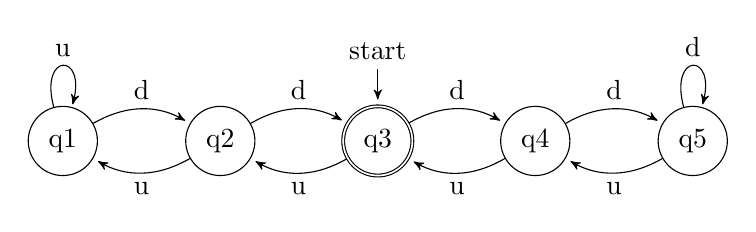
\begin{tikzpicture}[>=stealth',shorten >=2pt, auto, node distance=2cm]
	% Nodes {q1, q2, q3, q4, q5}
	\node [state] 											(q1) 				{q1};
	\node [state] 											(q2) [right of=q1]  {q2};
	\node [state, initial, initial where=above, accepting]  (q3) [right of=q2]  {q3};
	\node [state]											(q4) [right of=q3]  {q4};
	\node [state]   										(q5) [right of=q4]  {q5};

	% Paths
	\path [->] 	(q1) edge [loop above] node	{u}	(q1)
	            (q1) edge [bend left]  node {d} (q2)
				(q2) edge [bend left]  node {u} (q1)
				(q2) edge [bend left]  node {d} (q3)
				(q3) edge [bend left]  node {u} (q2)
				(q3) edge [bend left]  node {d} (q4)
				(q4) edge [bend left]  node {u} (q3)
				(q4) edge [bend left]  node {d} (q5)
				(q5) edge [bend left]  node {u} (q4)
				(q5) edge [loop above] node	{d}	(q5);
				
\end{tikzpicture} \\
\end{center}

%*********************************************************************************
% 1.4 here

\noindent
1.4: a, c, e, f, g.
For all parts, $\sum = \{a, b\} $

a. \{ w$|$ w has at least three a\textsc{\char13}s \}
\begin{center}
	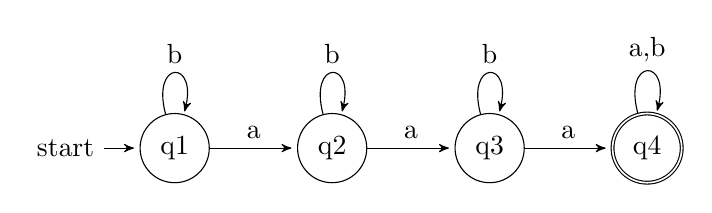
\begin{tikzpicture}[>=stealth',shorten >=2pt, auto, node distance=2cm]
	% Nodes {q1, q2, q3, q4, q5, etc}
	\node [state, initial] 		(q1) 				 {q1};
	\node [state] 				(q2)  [right of=q1]  {q2};
	\node [state]   			(q3)  [right of=q2]  {q3};
	\node [state, accepting]	(q4)  [right of=q3]  {q4};
	
	% Paths
	\path [->] 	(q1) edge 				node	{a}		(q2);
	\path [->] 	(q1) edge [loop above] 	node	{b}		(q1);
	\path [->] 	(q2) edge 				node	{a}		(q3);
	\path [->] 	(q2) edge [loop above] 	node	{b}		(q2);
	\path [->] 	(q3) edge 				node	{a}		(q4);
	\path [->] 	(q3) edge [loop above] 	node	{b}		(q3);
	\path [->] 	(q4) edge [loop above] 	node	{a,b}	(q4);
	
	\end{tikzpicture} \\
\end{center}

\clearpage
\{ w$|$ w has at least two b\textsc{\char13}s \}
\begin{center}
	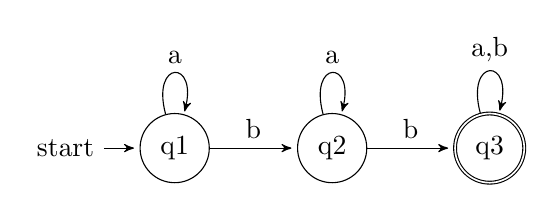
\begin{tikzpicture}[>=stealth',shorten >=2pt, auto, node distance=2cm]
	% Nodes {q1, q2, q3, q4, q5, etc}
	\node [state, initial] 		(q1) 				 {q1};
	\node [state] 				(q2)  [right of=q1]  {q2};
	\node [state, accepting]	(q3)  [right of=q2]  {q3};
	
	% Paths
	\path [->] 	(q1) edge 				node	{b}		(q2);
	\path [->] 	(q1) edge [loop above] 	node	{a}		(q1);
	\path [->] 	(q2) edge 				node	{b}		(q3);
	\path [->] 	(q2) edge [loop above] 	node	{a}		(q2);
	\path [->] 	(q3) edge [loop above] 	node	{a,b}	(q3);
	
	\end{tikzpicture} \\
\end{center}

\{w$|$ w has at least three a’s and at least two b’s\}
\begin{center}
	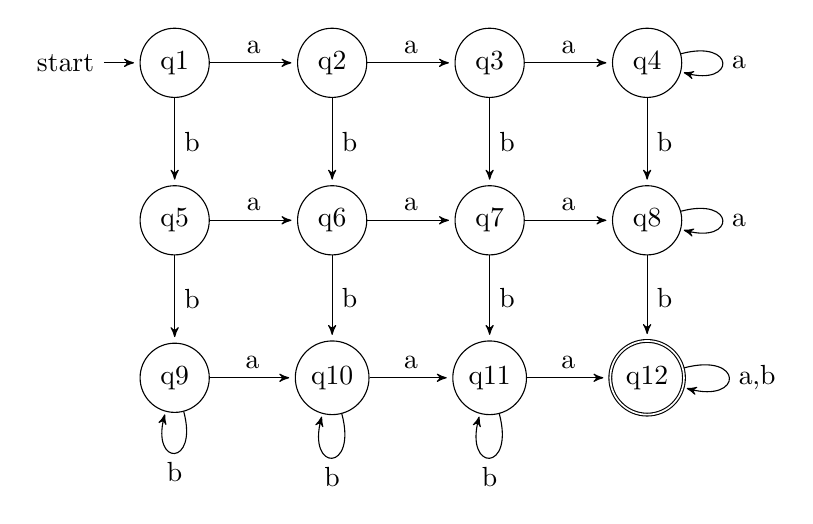
\begin{tikzpicture}[>=stealth',shorten >=2pt, auto, node distance=2cm]
	% Nodes {q1, q2, q3, q4, q5, etc}
	\node [state, initial] 		(q1) 				 {q1};
	\node [state] 				(q2)  [right of=q1]  {q2};
	\node [state]   			(q3)  [right of=q2]  {q3};
	\node [state]				(q4)  [right of=q3]  {q4};
	\node [state]   			(q5)  [below of=q1]  {q5};
	\node [state]   			(q6)  [below of=q2]  {q6};
	\node [state]   			(q7)  [below of=q3]  {q7};
	\node [state]   			(q8)  [below of=q4]  {q8};
	\node [state]   			(q9)  [below of=q5]  {q9};
	\node [state]   			(q10) [below of=q6]  {q10};
	\node [state]   			(q11) [below of=q7]  {q11};
	\node [state, accepting]   	(q12) [below of=q8]  {q12};
	
	% Paths for first row
	\path [->] 	(q1) edge 				node	{a}	(q2);
	\path [->] 	(q1) edge 				node	{b}	(q5);
	\path [->] 	(q2) edge 				node	{a}	(q3);
	\path [->] 	(q2) edge 				node	{b}	(q6);
	\path [->] 	(q3) edge 				node	{a}	(q4);
	\path [->] 	(q3) edge 				node	{b}	(q7);
	\path [->] 	(q4) edge [loop right] 	node	{a}	(q4);
	\path [->] 	(q4) edge 				node	{b}	(q8);
	
	% Paths for second row
	\path [->] 	(q5) edge			 	node	{a}	(q6);
	\path [->] 	(q5) edge 				node	{b}	(q9);
	\path [->] 	(q6) edge 				node	{a}	(q7);
	\path [->] 	(q6) edge 				node	{b}	(q10);
	\path [->] 	(q7) edge 				node	{a}	(q8);
	\path [->] 	(q7) edge 				node	{b}	(q11);
	\path [->] 	(q8) edge [loop right] 	node	{a}	(q8);
	\path [->] 	(q8) edge 				node	{b}	(q12);
	
	% Paths for third row
	\path [->] 	(q9)  edge 				node  {a} 	(q10);
	\path [->] 	(q9)  edge [loop below] node  {b} 	(q9);
	\path [->] 	(q10) edge 				node  {a} 	(q11);
	\path [->] 	(q10) edge [loop below] node  {b} 	(q10);
	\path [->] 	(q11) edge 				node  {a} 	(q12);
	\path [->] 	(q11) edge [loop below]	node  {b} 	(q11);
	\path [->] 	(q12) edge [loop right] node  {a,b}	(q12);

	\end{tikzpicture} \\
\end{center}

c. \{ w$|$ w has an even number of a\textsc{\char13}s \}
\begin{center}
	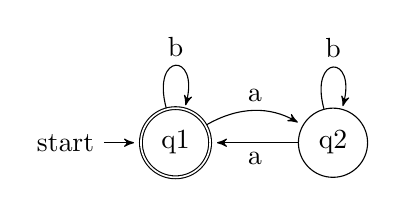
\begin{tikzpicture}[>=stealth',shorten >=2pt, auto, node distance=2cm]
	% Nodes {q1, q2, q3, q4, q5, etc}
	\node [state, initial, accepting] 		(q1) 				 {q1};
	\node [state] 							(q2)  [right of=q1]  {q2};
	
	% Paths
	\path [->] 	(q1) edge [bend left]	node	{a}		(q2);
	\path [->] 	(q1) edge [loop above] 	node	{b}		(q1);
	\path [->] 	(q2) edge				node	{a}		(q1);
	\path [->] 	(q2) edge [loop above] 	node	{b}		(q2);
	
	\end{tikzpicture} \\
\end{center}

\{ w$|$ w has one or two b\textsc{\char13}s \}
\begin{center}
	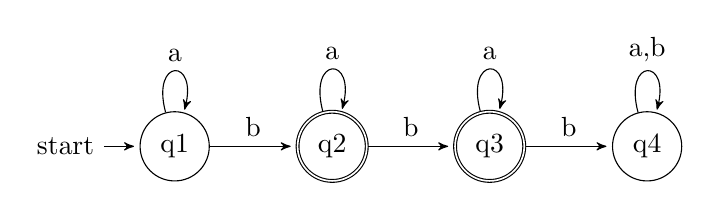
\begin{tikzpicture}[>=stealth',shorten >=2pt, auto, node distance=2cm]
	% Nodes {q1, q2, q3, q4, q5, etc}
	\node [state, initial] 		(q1) 				 {q1};
	\node [state, accepting] 	(q2)  [right of=q1]  {q2};
	\node [state, accepting]    (q3)  [right of=q2]  {q3};
	\node [state]				(q4)  [right of=q3]  {q4};
	
	% Paths
	\path [->] 	(q1) edge 				node	{b}		(q2);
	\path [->] 	(q1) edge [loop above] 	node	{a}		(q1);
	\path [->] 	(q2) edge 				node	{b}		(q3);
	\path [->] 	(q2) edge [loop above] 	node	{a}		(q2);
	\path [->] 	(q3) edge 				node	{b}		(q4);
	\path [->] 	(q3) edge [loop above] 	node	{a}		(q3);
	\path [->] 	(q4) edge [loop above] 	node	{a,b}	(q4);
	
	\end{tikzpicture} \\
\end{center}

\clearpage
\{ w$|$ w has an even number of a\textsc{\char13}s
and one or two b\textsc{\char13}s \}
\begin{center}
	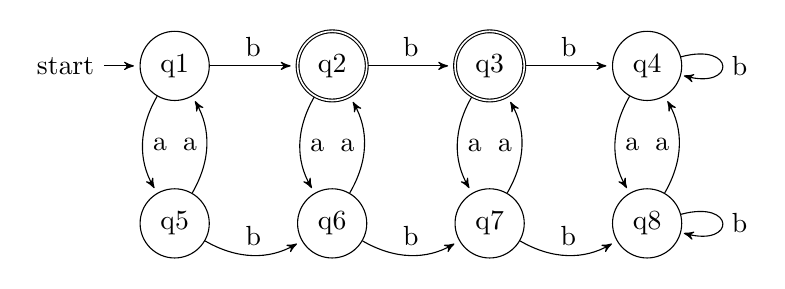
\begin{tikzpicture}[>=stealth',shorten >=2pt, auto, node distance=2cm]
	% Nodes {q1, q2, q3, q4, q5, etc}
	\node [state, initial] 		(q1) 				 {q1};
	\node [state, accepting] 	(q2)  [right of=q1]  {q2};
	\node [state, accepting]    (q3)  [right of=q2]  {q3};
	\node [state]				(q4)  [right of=q3]  {q4};
	\node [state]				(q5)  [below of=q1]  {q5};
	\node [state]				(q6)  [below of=q2]  {q6};
	\node [state]				(q7)  [below of=q3]  {q7};
	\node [state]				(q8)  [below of=q4]  {q8};
	
	% Paths
	\path [->] 	(q1) edge 				node	{b}		(q2);
	\path [->] 	(q1) edge [bend right]	node	{a}		(q5);
	\path [->] 	(q2) edge 				node	{b}		(q3);
	\path [->] 	(q2) edge [bend right]	node	{a}		(q6);
	\path [->] 	(q3) edge 				node	{b}		(q4);
	\path [->] 	(q3) edge [bend right]	node	{a}		(q7);
	\path [->] 	(q4) edge [loop right] 	node	{b}		(q4);
	\path [->] 	(q4) edge [bend right]	node	{a}		(q8);
	\path [->] 	(q5) edge [bend right]	node	{a}		(q1);
	\path [->] 	(q5) edge [bend right]	node	{b}		(q6);
	\path [->] 	(q6) edge [bend right]	node	{a}		(q2);
	\path [->] 	(q6) edge [bend right]	node	{b}		(q7);
	\path [->] 	(q7) edge [bend right]	node	{a}		(q3);
	\path [->] 	(q7) edge [bend right]	node	{b}		(q8);
	\path [->] 	(q8) edge [bend right]	node	{a}		(q4);
	\path [->] 	(q8) edge [loop right]	node	{b}		(q8);
	
	\end{tikzpicture} \\
\end{center}

e. \{ w$|$ w starts with an a \}
\begin{center}
	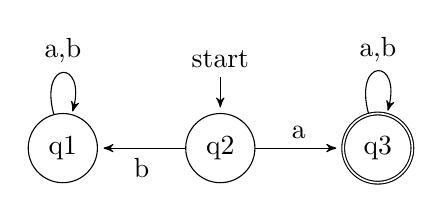
\begin{tikzpicture}[>=stealth',shorten >=2pt, auto, node distance=2cm]
	% Nodes {q1, q2, q3, q4, q5, etc}
	\node [state] 									(q1) 				 {q1};
	\node [state, initial, initial where=above] 	(q2)  [right of=q1]  {q2};
	\node [state, accepting]						(q3)  [right of=q2]  {q3};
	
	% Paths
	\path [->] 	(q1) edge [loop above] 	node	{a,b}	(q1);
	\path [->] 	(q2) edge 				node	{b}		(q1);
	\path [->] 	(q2) edge 				node	{a}		(q3);
	\path [->] 	(q3) edge [loop above] 	node	{a,b}	(q3);
	
	\end{tikzpicture} \\
\end{center}

\{ w$|$ w has at most one b \}
\begin{center}
	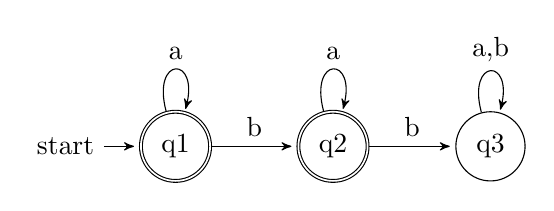
\begin{tikzpicture}[>=stealth',shorten >=2pt, auto, node distance=2cm]
	% Nodes {q1, q2, q3, q4, q5, etc}
	\node [state, initial,accepting] 	(q1) 				 {q1};
	\node [state, accepting] 			(q2)  [right of=q1]  {q2};
	\node [state]						(q3)  [right of=q2]  {q3};
	
	% Paths
	\path [->] 	(q1) edge [loop above] 	node	{a}     (q1);
	\path [->] 	(q1) edge 				node	{b}		(q2);
    \path [->] 	(q2) edge [loop above] 	node	{a}     (q2);
	\path [->] 	(q2) edge 				node	{b}		(q3);
	\path [->] 	(q3) edge [loop above] 	node	{a,b}	(q3);
	
	\end{tikzpicture} \\
\end{center}

\{ w$|$ w starts with an a and has at most one b \}
\begin{center}
	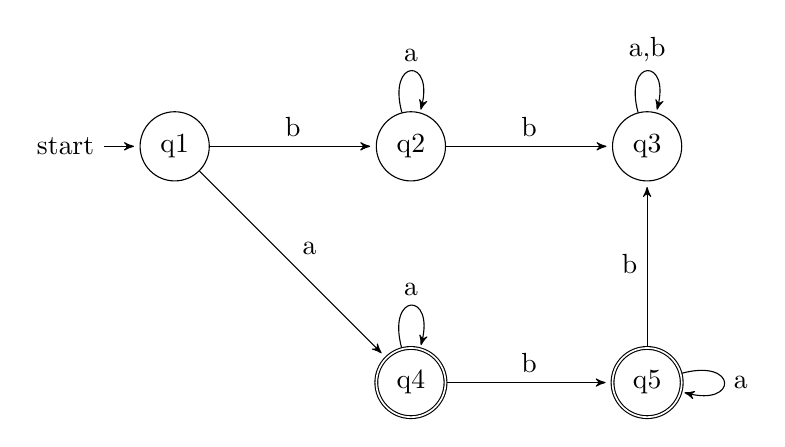
\begin{tikzpicture}[>=stealth',shorten >=2pt, auto, node distance=3cm]
	% Nodes {q1, q2, q3, q4, q5, etc}
	\node [state, initial] 		(q1) 				 {q1};
	\node [state] 				(q2)  [right of=q1]  {q2};
	\node [state]    			(q3)  [right of=q2]  {q3};
	\node [state, accepting]	(q4)  [below of=q2]  {q4};
	\node [state, accepting]	(q5)  [below of=q3]  {q5};
	
	% Paths
	\path [->] 	(q1) edge 				node	{b}		(q2);
	\path [->] 	(q1) edge 				node	{a}		(q4);
	\path [->] 	(q2) edge 				node	{b}		(q3);
	\path [->] 	(q2) edge [loop above] 	node	{a}		(q2);
	\path [->] 	(q3) edge [loop above] 	node	{a,b}	(q3);
	\path [->] 	(q4) edge [loop above] 	node	{a}		(q4);
	\path [->] 	(q4) edge 				node	{b}		(q5);
	\path [->] 	(q5) edge 				node	{b}		(q3);
	\path [->] 	(q5) edge [loop right] 	node	{a}		(q5);
	
	\end{tikzpicture} \\
\end{center}

\clearpage
f. \{ w$|$ w has an odd number of a\textsc{\char13}s \}
\begin{center}
    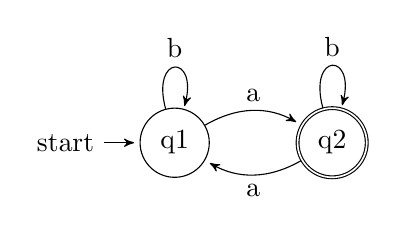
\begin{tikzpicture}[>=stealth',shorten >=2pt, auto, node distance=2cm]
    % Nodes {q1, q2, q3, q4, q5, etc}
    \node [state, initial] 	    (q1) 				 {q1};
    \node [state, accepting]    (q2)  [right of=q1]  {q2};
    
    % Paths
    \path [->] 	(q1) edge [loop above] 	node	{b}     (q1);
    \path [->] 	(q1) edge [bend left]   node	{a}		(q2);
    \path [->] 	(q2) edge [loop above] 	node	{b}     (q2);
    \path [->] 	(q2) edge [bend left] 	node	{a}		(q1);
    
    \end{tikzpicture} \\
\end{center}

\{ w$|$ w ends with a b \}
\begin{center}
    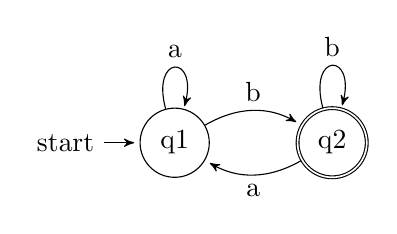
\begin{tikzpicture}[>=stealth',shorten >=2pt, auto, node distance=2cm]
    % Nodes {q1, q2, q3, q4, q5, etc}
    \node [state, initial] 	    (q1) 				 {q1};
    \node [state, accepting]    (q2)  [right of=q1]  {q2};
    
    % Paths
    \path [->] 	(q1) edge [loop above] 	node	{a}     (q1);
    \path [->] 	(q1) edge [bend left]   node	{b}		(q2);
    \path [->] 	(q2) edge [loop above] 	node	{b}     (q2);
    \path [->] 	(q2) edge [bend left] 	node	{a}		(q1);
    
    \end{tikzpicture} \\
\end{center}

\{ w$|$ w has an odd number of a\textsc{\char13}s and ends with a b \}
\begin{center}
    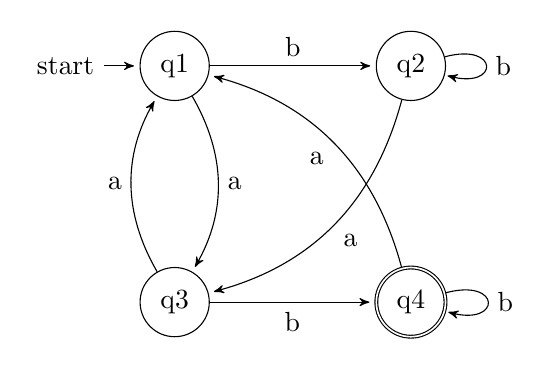
\begin{tikzpicture}[>=stealth',shorten >=2pt, auto, node distance=3cm]
    % Nodes {q1, q2, q3, q4, q5, etc}
    \node [state, initial] 	    (q1) 				 {q1};
    \node [state] 	            (q2)  [right of=q1]  {q2};
    \node [state] 	            (q3)  [below of=q1]  {q3};
    \node [state, accepting]    (q4)  [below of=q2]  {q4};
    
    % Paths
    \path [->] 	(q1) edge           	node	        {b}     (q2);
    \path [->] 	(q1) edge [bend left]   node	        {a}     (q3);
    \path [->] 	(q2) edge [loop right] 	node	        {b}     (q2);
    \path [->] 	(q2) edge [bend left]	node	        {a}		(q3);
    \path [->] 	(q3) edge [bend left]   node	        {a}     (q1);
    \path [->] 	(q3) edge               node [below]	{b}     (q4);
    \path [->] 	(q4) edge [loop right] 	node	        {b}     (q4);
    \path [->] 	(q4) edge [bend right]	node	        {a}		(q1);
    
    \end{tikzpicture} \\
\end{center}

g. \{ w$|$ w has even length \} \\
\begin{center}
    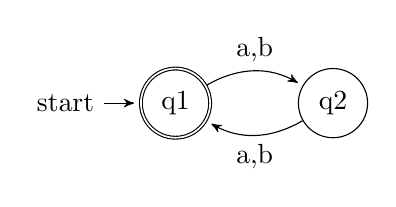
\begin{tikzpicture}[>=stealth',shorten >=2pt, auto, node distance=2cm]
    % Nodes {q1, q2, q3, q4, q5, etc}
    \node [state, initial, accepting] 	(q1) 				 {q1};
    \node [state]                       (q2)  [right of=q1]  {q2};
    
    % Paths
    \path [->] 	(q1) edge [bend left]   node	{a,b}		(q2);
    \path [->] 	(q2) edge [bend left] 	node	{a,b}		(q1);
    
    \end{tikzpicture} \\
\end{center}

\{ w$|$ w has an odd number of a\textsc{\char13}s \}
\begin{center}
    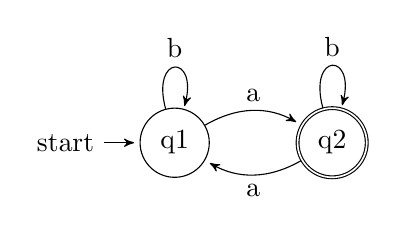
\begin{tikzpicture}[>=stealth',shorten >=2pt, auto, node distance=2cm]
    % Nodes {q1, q2, q3, q4, q5, etc}
    \node [state, initial] 	  (q1) 				   {q1};
    \node [state, accepting]  (q2)  [right of=q1]  {q2};
    
    % Paths
    \path [->] 	(q1) edge [bend left]   node	{a}		(q2);
    \path [->] 	(q1) edge [loop above] 	node	{b}     (q1);
    \path [->] 	(q2) edge [bend left] 	node	{a}		(q1);
    \path [->] 	(q2) edge [loop above] 	node	{b}     (q2);
    
    \end{tikzpicture} \\
\end{center}

\{ w$|$ w has even length and an odd number of a\textsc{\char13}s \}
\begin{center}
    \begin{tikzpicture}[>=stealth',shorten >=2pt, auto, node distance=3cm]
    % Nodes {q1, q2, q3, q4, q5, etc}
    \node [state, initial] 	  (q1) 				   {q1};
    \node [state] 	          (q2) 	[right of=q2]  {q2};
    \node [state] 	          (q3) 	[below of=q1]  {q3};
    \node [state, accepting]  (q4)  [below of=q2]  {q4};
    
    % Paths
    \path [->] 	(q1) edge [bend left]   node	        {b}		(q2);
    \path [->] 	(q1) edge [bend left] 	node	        {a}     (q3);
    \path [->] 	(q2) edge [bend left] 	node [above]	{b}		(q1);
    \path [->] 	(q2) edge [bend left] 	node	        {a}     (q4);
    \path [->] 	(q3) edge [bend left] 	node	        {a}     (q1);
    \path [->] 	(q3) edge [bend left] 	node [below]    {b}     (q4);
    \path [->] 	(q4) edge [bend left] 	node	        {b}     (q3);
    \path [->] 	(q4) edge [bend left] 	node	        {a}     (q2);
    
    \end{tikzpicture} \\
\end{center}

%*********************************************************************************
% 1.5 here

\noindent
1.5: c, d, e, f, g, h. For all parts, $\sum = \{a, b\} $  \\
c. \{ w$|$ w contains neither the substrings ab nor ba \}

Simpler language \\
\begin{center}
    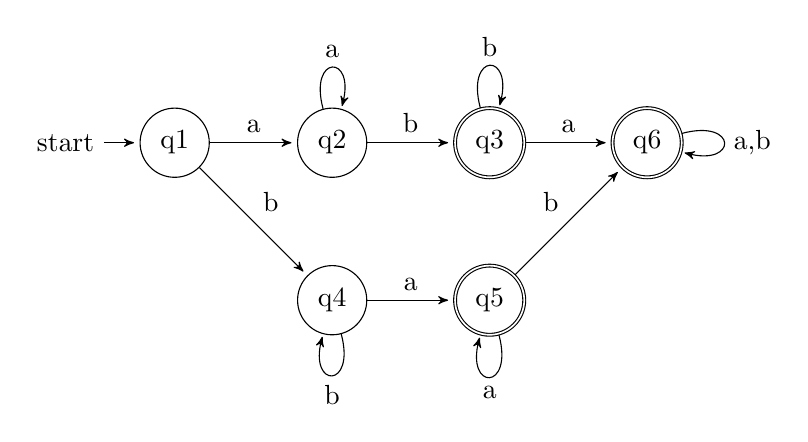
\begin{tikzpicture}[>=stealth',shorten >=2pt, auto, node distance=2cm]
    % Nodes {q1, q2, q3, q4, q5, etc}
    \node [state, initial] 		(q1) 				 {q1};
    \node [state] 	            (q2)  [right of=q1]  {q2};
    \node [state, accepting]    (q3)  [right of=q2]  {q3};
    \node [state]	            (q4)  [below of=q2]  {q4};
    \node [state, accepting]	(q5)  [below of=q3]  {q5};
    \node [state, accepting]	(q6)  [right of=q3]  {q6};
    
    % Paths
    \path [->] 	(q1) edge 				node	{a}		(q2);
    \path [->] 	(q1) edge 				node	{b}		(q4);
    \path [->] 	(q2) edge 				node	{b}		(q3);
    \path [->] 	(q2) edge [loop above]	node	{a}		(q2);
    \path [->] 	(q3) edge 				node	{a}		(q6);
    \path [->] 	(q3) edge [loop above]	node	{b}		(q3);
    \path [->] 	(q4) edge 				node	{a}		(q5);
    \path [->] 	(q4) edge [loop below]	node	{b}		(q4);
    \path [->] 	(q5) edge 				node	{b}		(q6);
    \path [->] 	(q5) edge [loop below]	node	{a}		(q5);
    \path [->] 	(q6) edge [loop right]	node	{a,b}	(q6);
    
    \end{tikzpicture} \\
\end{center}

\clearpage
Language given. \\
\begin{center}
    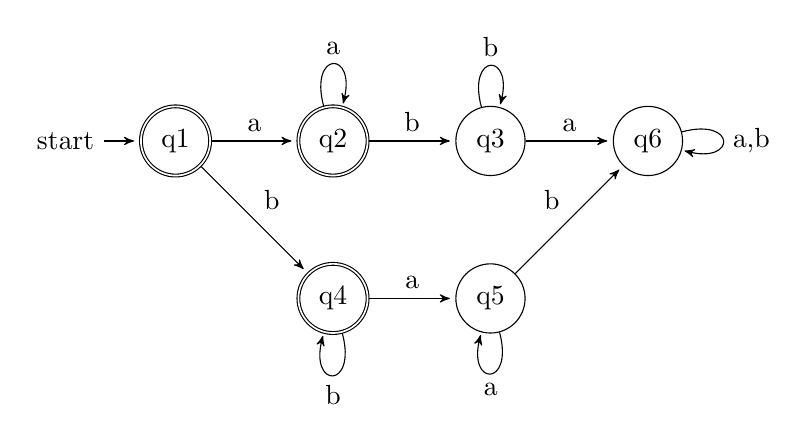
\begin{tikzpicture}[>=stealth',shorten >=2pt, auto, node distance=2cm]
    % Nodes {q1, q2, q3, q4, q5, etc}
    \node [state, initial, accepting] 		(q1) 				 {q1};
    \node [state, accepting] 	            (q2)  [right of=q1]  {q2};
    \node [state]                           (q3)  [right of=q2]  {q3};
    \node [state, accepting]	            (q4)  [below of=q2]  {q4};
    \node [state]	                        (q5)  [below of=q3]  {q5};
    \node [state]	                        (q6)  [right of=q3]  {q6};
    
    % Paths
    \path [->] 	(q1) edge 				node	{a}		(q2);
    \path [->] 	(q1) edge 				node	{b}		(q4);
    \path [->] 	(q2) edge 				node	{b}		(q3);
    \path [->] 	(q2) edge [loop above]	node	{a}		(q2);
    \path [->] 	(q3) edge 				node	{a}		(q6);
    \path [->] 	(q3) edge [loop above]	node	{b}		(q3);
    \path [->] 	(q4) edge 				node	{a}		(q5);
    \path [->] 	(q4) edge [loop below]	node	{b}		(q4);
    \path [->] 	(q5) edge 				node	{b}		(q6);
    \path [->] 	(q5) edge [loop below]	node	{a}		(q5);
    \path [->] 	(q6) edge [loop right]	node	{a,b}	(q6);
    
    \end{tikzpicture} \\
\end{center}

\noindent
d. \{ w$|$ w is any string not in a*b* \} \\ 
Simpler language \\
\begin{center}
    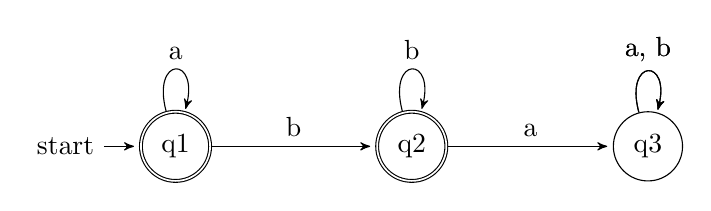
\begin{tikzpicture}[>=stealth',shorten >=2pt, auto, node distance=3cm]
    % Nodes {q1, q2, q3, q4, q5, etc}
    \node [state, initial, accepting] 		(q1) 				 {q1};
    \node [state, accepting] 	            (q2)  [right of=q1]  {q2};
    \node [state]                           (q3)  [right of=q2]  {q3};
    
    % Paths
    \path [->] 	(q1) edge 				node	{b}		(q2);
    \path [->] 	(q1) edge [loop above] 	node	{a}	    (q1);
    \path [->] 	(q2) edge 				node	{a}		(q3);
    \path [->] 	(q2) edge [loop above] 	node	{b}	    (q2);
    \path [->] 	(q3) edge [loop above] 	node	{a, b}	(q3);
    \path [->] 	(q3) edge [loop above] 	node	{a, b}	(q3);
    
    \end{tikzpicture} \\
\end{center}

Language given \\
\begin{center}
    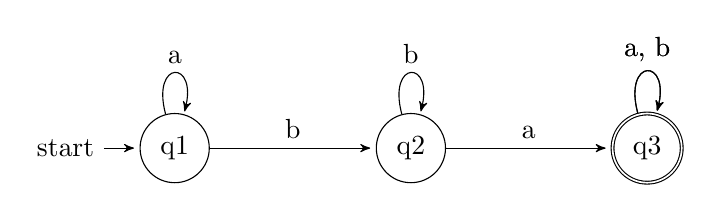
\begin{tikzpicture}[>=stealth',shorten >=2pt, auto, node distance=3cm]
    % Nodes {q1, q2, q3, q4, q5, etc}
    \node [state, initial] 		(q1) 				 {q1};
    \node [state] 	            (q2)  [right of=q1]  {q2};
    \node [state, accepting]    (q3)  [right of=q2]  {q3};
    
    % Paths
    \path [->] 	(q1) edge 				node	{b}		(q2);
    \path [->] 	(q1) edge [loop above] 	node	{a}	    (q1);
    \path [->] 	(q2) edge 				node	{a}		(q3);
    \path [->] 	(q2) edge [loop above] 	node	{b}	    (q2);
    \path [->] 	(q3) edge [loop above] 	node	{a, b}	(q3);
    \path [->] 	(q3) edge [loop above] 	node	{a, b}	(q3);
    
    \end{tikzpicture} \\
\end{center}

\clearpage
\noindent
e. \{ w$|$ w is any string not in (ab\textsuperscript{+})* \} \\
Simpler language
\begin{center}
    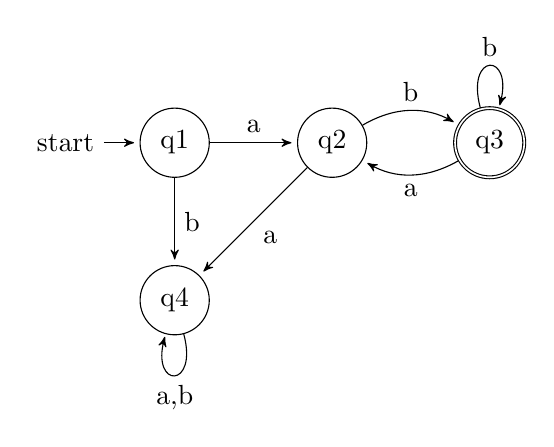
\begin{tikzpicture}[>=stealth',shorten >=2pt, auto, node distance=2cm]
    % Nodes {q1, q2, q3, q4, q5, etc}
    \node [state, initial] 		(q1) 				 {q1};
    \node [state] 	            (q2)  [right of=q1]  {q2};
    \node [state, accepting]    (q3)  [right of=q2]  {q3};
    \node [state]				(q4)  [below of=q1]  {q4};
    
    % Paths
    \path [->] 	(q1) edge 				node	{a}		(q2);
    \path [->] 	(q1) edge 				node	{b}		(q4);
    \path [->] 	(q2) edge [bend left]	node	{b}		(q3);
    \path [->] 	(q2) edge 				node	{a}		(q4);
    \path [->] 	(q3) edge [bend left]	node	{a}		(q2);
    \path [->] 	(q3) edge [loop above] 	node	{b}		(q3);
    \path [->] 	(q4) edge [loop below] 	node	{a,b}	(q4);
    
    \end{tikzpicture} \\
\end{center}

Language given
\begin{center}
    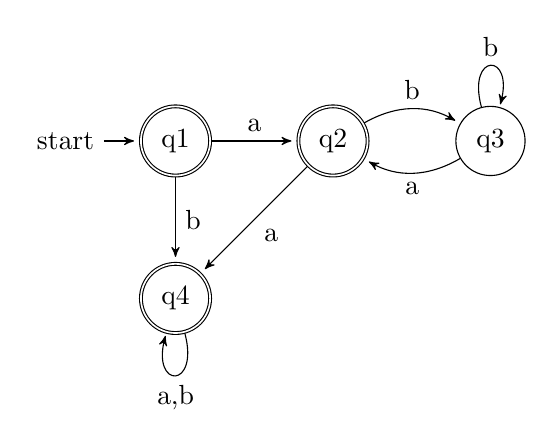
\begin{tikzpicture}[>=stealth',shorten >=2pt, auto, node distance=2cm]
    % Nodes {q1, q2, q3, q4, q5, etc}
    \node [state, initial, accepting] 		(q1) 				 {q1};
    \node [state, accepting] 	            (q2)  [right of=q1]  {q2};
    \node [state]                           (q3)  [right of=q2]  {q3};
    \node [state, accepting]				(q4)  [below of=q1]  {q4};
    
    % Paths
    \path [->] 	(q1) edge 				node	{a}		(q2);
    \path [->] 	(q1) edge 				node	{b}		(q4);
    \path [->] 	(q2) edge [bend left]	node	{b}		(q3);
    \path [->] 	(q2) edge 				node	{a}		(q4);
    \path [->] 	(q3) edge [bend left]	node	{a}		(q2);
    \path [->] 	(q3) edge [loop above] 	node	{b}		(q3);
    \path [->] 	(q4) edge [loop below] 	node	{a,b}	(q4);
    
    \end{tikzpicture} \\
\end{center}

\clearpage
\noindent
f. \{ w $|$ w is any string not in a* $\bigcup$ b* \} \\
Simpler language
\begin{center}
    \begin{tikzpicture}[>=stealth',shorten >=2pt, auto, node distance=3cm]
    % Nodes {q1, q2, q3, q4, q5, etc}
    \node [state, initial, accepting] 		(q1) 				 {q1};
    \node [state, accepting] 	            (q2)  [right of=q1]  {q2};
    \node [state]                           (q3)  [right of=q2]  {q3};
    \node [state, accepting]				(q4)  [below of=q2]  {q4};
    
    % Paths
    \path [->] 	(q1) edge 				node	{a}		(q2);
    \path [->] 	(q1) edge 				node	{b}		(q4);
    \path [->] 	(q2) edge           	node	{b}		(q3);
    \path [->] 	(q2) edge [loop above] 	node	{a}	    (q2);
    \path [->] 	(q3) edge [loop right] 	node	{a,b}   (q3);
    \path [->] 	(q4) edge [loop below] 	node	{b}	    (q4);
    \path [->] 	(q4) edge 				node	{a}		(q3);
    
    \end{tikzpicture} \\
\end{center}

Language given
\begin{center}
    \begin{tikzpicture}[>=stealth',shorten >=2pt, auto, node distance=3cm]
    % Nodes {q1, q2, q3, q4, q5, etc}
    \node [state, initial] 		(q1) 				 {q1};
    \node [state] 	            (q2)  [right of=q1]  {q2};
    \node [state, accepting]    (q3)  [right of=q2]  {q3};
    \node [state]				(q4)  [below of=q2]  {q4};
    
    % Paths
    \path [->] 	(q1) edge 				node	{a}		(q2);
    \path [->] 	(q1) edge 				node	{b}		(q4);
    \path [->] 	(q2) edge           	node	{b}		(q3);
    \path [->] 	(q2) edge [loop above] 	node	{a}	    (q2);
    \path [->] 	(q3) edge [loop right] 	node	{a,b}   (q3);
    \path [->] 	(q4) edge [loop below] 	node	{b}	    (q4);
    \path [->] 	(q4) edge 				node	{a}		(q3);
    
    \end{tikzpicture} \\
\end{center}

\noindent
g. \{ w$|$ w is any string that doesn\textsc{\char13}t contain exactly two a\textsc{\char13}s \} \\
Simpler language
\begin{center}
    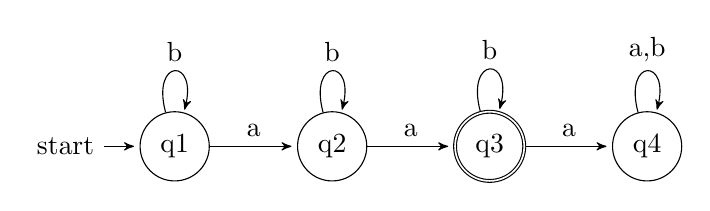
\begin{tikzpicture}[>=stealth',shorten >=2pt, auto, node distance=2cm]
    % Nodes {q1, q2, q3, q4, q5, etc}
    \node [state, initial] 		(q1) 				 {q1};
    \node [state] 				(q2)  [right of=q1]  {q2};
    \node [state, accepting]   	(q3)  [right of=q2]  {q3};
    \node [state]	            (q4)  [right of=q3]  {q4};
    
    % Paths
    \path [->] 	(q1) edge 				node	{a}		(q2);
    \path [->] 	(q1) edge [loop above] 	node	{b}		(q1);
    \path [->] 	(q2) edge 				node	{a}		(q3);
    \path [->] 	(q2) edge [loop above] 	node	{b}		(q2);
    \path [->] 	(q3) edge 				node	{a}		(q4);
    \path [->] 	(q3) edge [loop above] 	node	{b}		(q3);
    \path [->] 	(q4) edge [loop above] 	node	{a,b}	(q4);
    
    \end{tikzpicture} \\
\end{center}

Language given
\begin{center}
    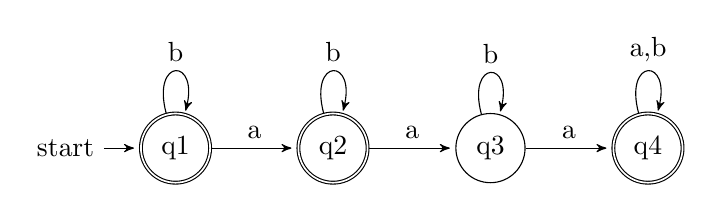
\begin{tikzpicture}[>=stealth',shorten >=2pt, auto, node distance=2cm]
    % Nodes {q1, q2, q3, q4, q5, etc}
    \node [state, initial, accepting] 		(q1) 				 {q1};
    \node [state, accepting] 				(q2)  [right of=q1]  {q2};
    \node [state]   	                    (q3)  [right of=q2]  {q3};
    \node [state, accepting]	            (q4)  [right of=q3]  {q4};
    
    % Paths
    \path [->] 	(q1) edge 				node	{a}		(q2);
    \path [->] 	(q1) edge [loop above] 	node	{b}		(q1);
    \path [->] 	(q2) edge 				node	{a}		(q3);
    \path [->] 	(q2) edge [loop above] 	node	{b}		(q2);
    \path [->] 	(q3) edge 				node	{a}		(q4);
    \path [->] 	(q3) edge [loop above] 	node	{b}		(q3);
    \path [->] 	(q4) edge [loop above] 	node	{a,b}	(q4);
    
    \end{tikzpicture} \\
\end{center}

\noindent
h. \{ w$|$ w is any string except a and b \} \\
Simpler language
\begin{center}
    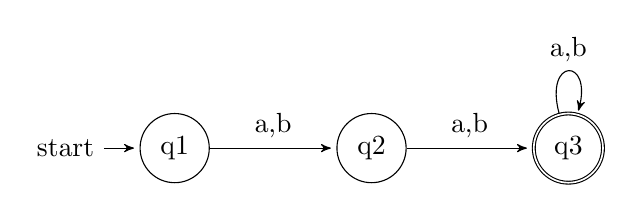
\begin{tikzpicture}[>=stealth',shorten >=2pt, auto, node distance=2.5cm]
    % Nodes {q1, q2, q3, q4, q5, etc}
    \node [state, initial] 		(q1) 				 {q1};
    \node [state] 				(q2)  [right of=q1]  {q2};
    \node [state, accepting]   	(q3)  [right of=q2]  {q3};
    
    % Paths
    \path [->] 	(q1) edge 				node	{a,b}		(q2);
    \path [->] 	(q2) edge 				node	{a,b}		(q3);
    \path [->] 	(q3) edge [loop above] 	node	{a,b}		(q3);
    
    \end{tikzpicture} \\
\end{center}

Language given
\begin{center}
    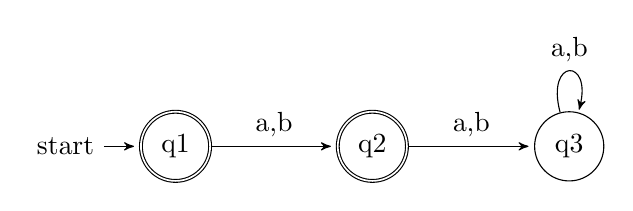
\begin{tikzpicture}[>=stealth',shorten >=2pt, auto, node distance=2.5cm]
    % Nodes {q1, q2, q3, q4, q5, etc}
    \node [state, initial, accepting] 		(q1) 				 {q1};
    \node [state, accepting] 				(q2)  [right of=q1]  {q2};
    \node [state]   	                    (q3)  [right of=q2]  {q3};
    
    % Paths
    \path [->] 	(q1) edge 				node	{a,b}		(q2);
    \path [->] 	(q2) edge 				node	{a,b}		(q3);
    \path [->] 	(q3) edge [loop above] 	node	{a,b}		(q3);
    
    \end{tikzpicture} \\
\end{center}

%*********************************************************************************
% 1.6 here

\noindent
1.6: a, b, c, d, e, f, g, h, I, j, k, l, m, n \\
a. \{w$|$ w begins with a 1 and ends with a 0\}
\begin{center}
    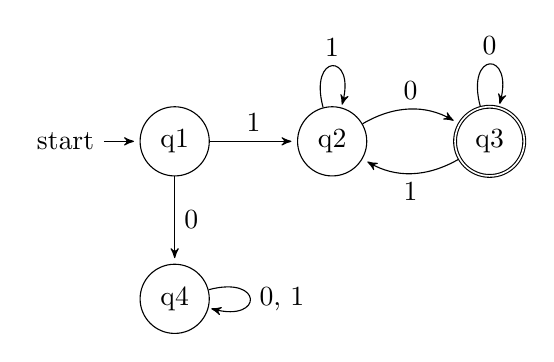
\begin{tikzpicture}[>=stealth',shorten >=2pt, auto, node distance=2cm]
    % Nodes {q1, q2, q3, q4, q5, etc}
    \node [state, initial]    	(q1) 				 {q1};
    \node [state] 				(q2)  [right of=q1]  {q2};
    \node [state, accepting]   	(q3)  [right of=q2]  {q3};
    \node [state]	            (q4)  [below of=q1]  {q4};
    
    % Paths
    \path [->] 	(q1) edge 				node	{1}		(q2);
    \path [->] 	(q1) edge 				node	{0}		(q4);
    \path [->] 	(q2) edge [bend left]	node	{0}		(q3);
    \path [->] 	(q2) edge [loop above] 	node	{1}		(q2);
    \path [->] 	(q3) edge [bend left]	node	{1}		(q2);
    \path [->] 	(q3) edge [loop above] 	node	{0}		(q3);
    \path [->] 	(q4) edge [loop right] 	node	{0, 1}	(q4);
    
    \end{tikzpicture} \\
\end{center}

\clearpage
\noindent
b. \{w$|$ w contains at least three 1s\}
\begin{center}
    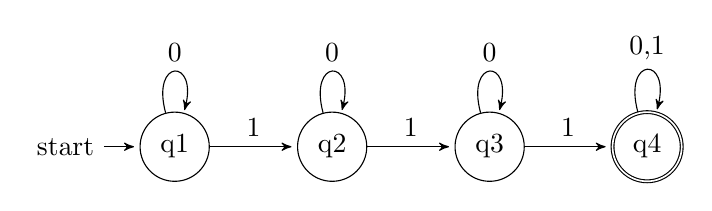
\begin{tikzpicture}[>=stealth',shorten >=2pt, auto, node distance=2cm]
    % Nodes {q1, q2, q3, q4, q5, etc}
    \node [state, initial] 		(q1) 				 {q1};
    \node [state] 				(q2)  [right of=q1]  {q2};
    \node [state]   	        (q3)  [right of=q2]  {q3};
    \node [state, accepting]	(q4)  [right of=q3]  {q4};
    
    % Paths
    \path [->] 	(q1) edge 				node	{1}		(q2);
    \path [->] 	(q1) edge [loop above] 	node	{0}		(q1);
    \path [->] 	(q2) edge 				node	{1}		(q3);
    \path [->] 	(q2) edge [loop above] 	node	{0}		(q2);
    \path [->] 	(q3) edge 				node	{1}		(q4);
    \path [->] 	(q3) edge [loop above] 	node	{0}		(q3);
    \path [->] 	(q4) edge [loop above] 	node	{0,1}	(q4);
    
    \end{tikzpicture} \\
\end{center}

\noindent
c. \{w$|$ w contains the substring 0101 (i.e., w = x0101y for some x and y)\}
\begin{center}
    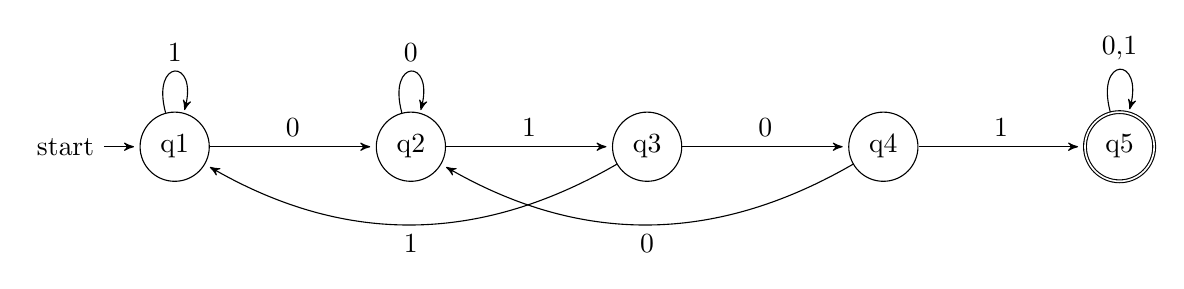
\begin{tikzpicture}[>=stealth',shorten >=2pt, auto, node distance=3cm]
    % Nodes {q1, q2, q3, q4, q5, etc}
    \node [state, initial] 		(q1) 				 {q1};
    \node [state] 				(q2)  [right of=q1]  {q2};
    \node [state]   	        (q3)  [right of=q2]  {q3};
    \node [state]   	        (q4)  [right of=q3]  {q4};
    \node [state, accepting]	(q5)  [right of=q4]  {q5};
    
    % Paths
    \path [->] 	(q1) edge 				node	{0}		(q2);
    \path [->] 	(q1) edge [loop above] 	node	{1}		(q1);
    \path [->] 	(q2) edge 				node	{1}		(q3);
    \path [->] 	(q2) edge [loop above] 	node	{0}		(q2);
    \path [->] 	(q3) edge 				node	{0}		(q4);
    \path [->] 	(q3) edge [bend left]	node	{1}		(q1);
    \path [->] 	(q4) edge 				node	{1}		(q5);
    \path [->] 	(q4) edge [bend left] 	node	{0}	    (q2);
    \path [->] 	(q5) edge [loop above] 	node	{0,1}		(q5);
    
    \end{tikzpicture} \\
\end{center}

\noindent
d. \{w$|$ w has length at least 3 and its third symbol is a 0\}
\begin{center}
    \begin{tikzpicture}[>=stealth',shorten >=2pt, auto, node distance=3cm]
    % Nodes {q1, q2, q3, q4, q5, etc}
    \node [state, initial] 		(q1) 				 {q1};
    \node [state] 				(q2)  [right of=q1]  {q2};
    \node [state]   	        (q3)  [right of=q2]  {q3};
    \node [state]   	        (q4)  [below of=q3]  {q4};
    \node [state, accepting]	(q5)  [right of=q3]  {q5};
    
    % Paths
    \path [->] 	(q1) edge 				node	{0,1}	(q2);
    \path [->] 	(q2) edge 				node	{0,1}	(q3);
    \path [->] 	(q3) edge 				node	{1}		(q4);
    \path [->] 	(q3) edge 				node	{0}		(q5);
    \path [->] 	(q4) edge [loop right] 	node	{0,1}   (q4);
    \path [->] 	(q5) edge [loop above] 	node	{0,1}   (q5);
    
    \end{tikzpicture} \\
\end{center}

\clearpage
\noindent
e. \{w$|$ w starts with 0 and has odd length, or starts with 1 and has even length\}
\begin{center}
    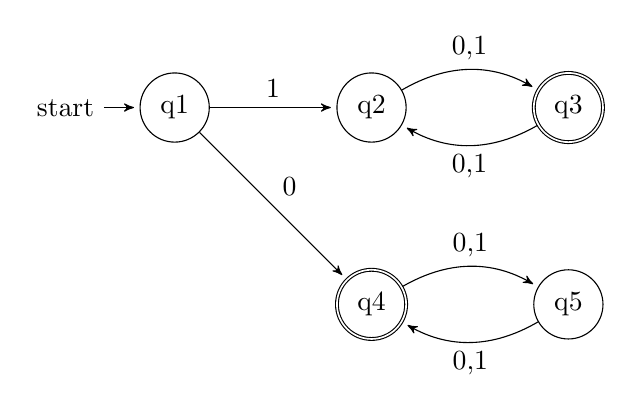
\begin{tikzpicture}[>=stealth',shorten >=2pt, auto, node distance=2.5cm]
    % Nodes {q1, q2, q3, q4, q5, etc}
    \node [state, initial] 		(q1) 				 {q1};
    \node [state] 	            (q2)  [right of=q1]  {q2};
    \node [state, accepting]    (q3)  [right of=q2]  {q3};
    \node [state, accepting]	(q4)  [below of=q2]  {q4};
    \node [state]	            (q5)  [below of=q3]  {q5};
    
    % Paths
    \path [->] 	(q1) edge 				node	{1}		(q2);
    \path [->] 	(q1) edge 				node	{0}		(q4);
    \path [->] 	(q2) edge [bend left]	node	{0,1}	(q3);
    \path [->] 	(q3) edge [bend left]	node	{0,1}	(q2);
    \path [->] 	(q4) edge [bend left]	node	{0,1}	(q5);
    \path [->] 	(q5) edge [bend left]	node	{0,1}	(q4);
    
    \end{tikzpicture} \\
\end{center}

\noindent
f. \{w$|$ w doesn’t contain the substring 110\}
\begin{center}
    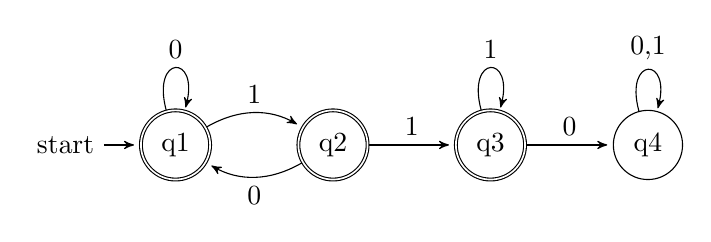
\begin{tikzpicture}[>=stealth',shorten >=2pt, auto, node distance=2cm]
    % Nodes {q1, q2, q3, q4, q5, etc}
    \node [state, initial, accepting] 		(q1) 				 {q1};
    \node [state, accepting] 				(q2)  [right of=q1]  {q2};
    \node [state, accepting]   	            (q3)  [right of=q2]  {q3};
    \node [state]	                        (q4)  [right of=q3]  {q4};
    
    % Paths
    \path [->] 	(q1) edge [bend left]	node	{1}		(q2);
    \path [->] 	(q1) edge [loop above] 	node	{0}		(q1);
    \path [->] 	(q2) edge [bend left]	node	{0}		(q1);
    \path [->] 	(q2) edge 				node	{1}		(q3);
    \path [->] 	(q3) edge 				node	{0}		(q4);
    \path [->] 	(q3) edge [loop above] 	node	{1}		(q3);
    \path [->] 	(q4) edge [loop above] 	node	{0,1}	(q4);
    
    \end{tikzpicture} \\
\end{center}

\noindent
g. \{w$|$ the length of w is at most 5\}
\begin{center}
    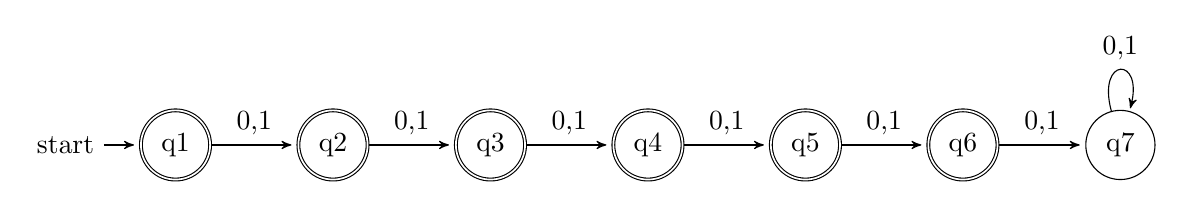
\begin{tikzpicture}[>=stealth',shorten >=2pt, auto, node distance=2cm]
    % Nodes {q1, q2, q3, q4, q5, etc}
    \node [state, initial, accepting] 		(q1) 				 {q1};
    \node [state, accepting] 				(q2)  [right of=q1]  {q2};
    \node [state, accepting]   	            (q3)  [right of=q2]  {q3};
    \node [state, accepting]   	            (q4)  [right of=q3]  {q4};
    \node [state, accepting]	            (q5)  [right of=q4]  {q5};
    \node [state, accepting]	            (q6)  [right of=q5]  {q6};
    \node [state]	                        (q7)  [right of=q6]  {q7};
    
    % Paths
    \path [->] 	(q1) edge 				node	{0,1}	(q2);
    \path [->] 	(q2) edge 				node	{0,1}	(q3);
    \path [->] 	(q3) edge 				node	{0,1}	(q4);
    \path [->] 	(q4) edge 				node	{0,1}	(q5);
    \path [->] 	(q5) edge 				node	{0,1}	(q6);
    \path [->] 	(q6) edge 				node	{0,1}	(q7);
    \path [->] 	(q7) edge [loop above] 	node	{0,1}   (q7);
    
    \end{tikzpicture} \\
\end{center}

\noindent
h. \{w$|$ w is any string except 11 and 111\}
\begin{center}
    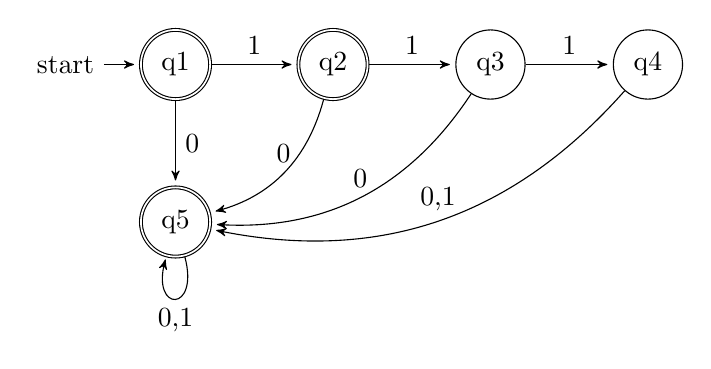
\begin{tikzpicture}[>=stealth',shorten >=2pt, auto, node distance=2cm]
    % Nodes {q1, q2, q3, q4, q5, etc}
    \node [state, initial, accepting] 	(q1) 				 {q1};
    \node [state, accepting] 			(q2)  [right of=q1]  {q2};
    \node [state]   	        		(q3)  [right of=q2]  {q3};
    \node [state]	            		(q4)  [right of=q3]  {q4};
    \node [state, accepting] 			(q5)  [below of=q1]  {q5};
    
    % Paths
    \path [->] 	(q1) edge	            node			{1}		(q2);
    \path [->] 	(q2) edge 				node			{1}		(q3);
    \path [->] 	(q3) edge 				node			{1}		(q4);
    \path [->] 	(q1) edge	            node			{0}		(q5);
    \path [->] 	(q2) edge [bend left]   node [above]	{0}		(q5);
    \path [->] 	(q3) edge [bend left]   node [above]	{0}		(q5);
    \path [->] 	(q4) edge [bend left]   node [above]	{0,1}	(q5);
    \path [->] 	(q5) edge [loop below] 	node			{0,1}	(q5);
    
    \end{tikzpicture} \\
\end{center}

\noindent
I. \{w$|$ every odd position of w is a 1\}
\begin{center}
    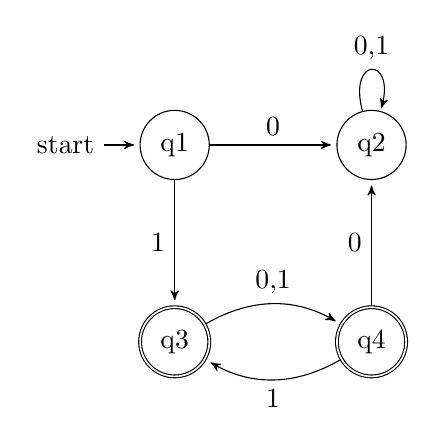
\begin{tikzpicture}[>=stealth',shorten >=2pt, auto, node distance=2.5cm]
    % Nodes {q1, q2, q3, q4, q5, etc}
    \node [state, initial] 		(q1) 				 {q1};
    \node [state] 		        (q2) [right of=q1]	 {q2};
    \node [state, accepting] 	(q3) [below of=q1]	 {q3};
    \node [state, accepting] 	(q4) [right of=q3]	 {q4};
    
    % Paths
    \path [->] 	(q1) edge 	            node	     {0}		(q2);
    \path [->] 	(q1) edge  				node [left]	 {1}		(q3);
    \path [->] 	(q2) edge [loop above]	node	     {0,1}	    (q2);
    \path [->] 	(q3) edge [bend left]   node	     {0,1}		(q4);
    \path [->] 	(q4) edge [bend left]   node	     {1}		(q3);
    \path [->] 	(q4) edge 	            node	     {0}		(q2);
    
    \end{tikzpicture} \\
\end{center}

\noindent
j. \{w$|$ w contains at least two 0s and at most one 1\}
\begin{center}
    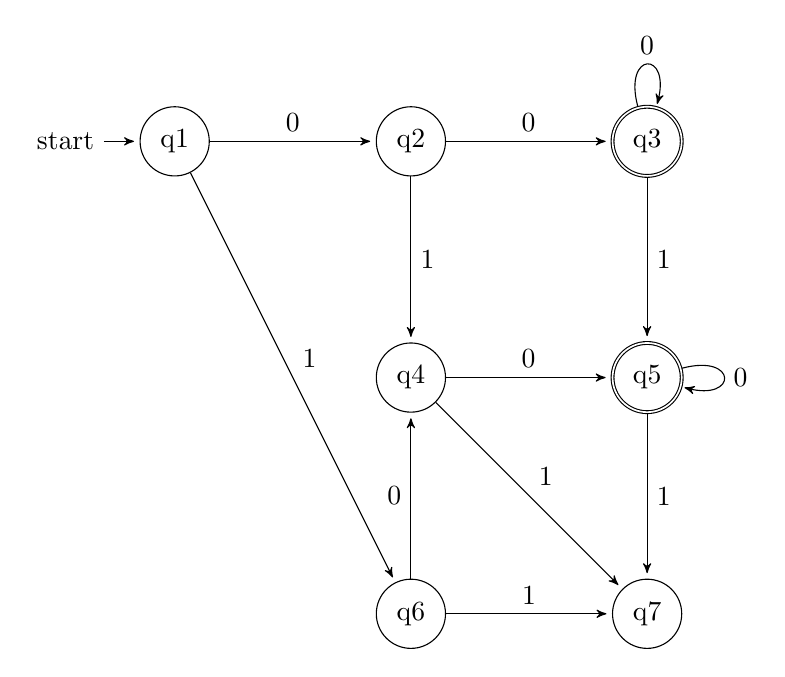
\begin{tikzpicture}[>=stealth',shorten >=2pt, auto, node distance=3cm]
    % Nodes {q1, q2, q3, q4, q5, etc}
    \node [state, initial] 		(q1) 				 {q1};
    \node [state] 				(q2)  [right of=q1]  {q2};
    \node [state, accepting]   	(q3)  [right of=q2]  {q3};
    \node [state] 	            (q4)  [below of=q2]  {q4};
    \node [state, accepting]    (q5)  [below of=q3]  {q5};
    \node [state] 	            (q6)  [below of=q4]  {q6};
    \node [state]               (q7)  [below of=q5]  {q7};
    
    % Paths
    \path [->] 	(q1) edge	            node	{0}		(q2);
    \path [->] 	(q1) edge	            node	{1}		(q6);
    \path [->] 	(q2) edge 				node	{0}		(q3);
    \path [->] 	(q2) edge 				node	{1}		(q4);
    \path [->] 	(q3) edge 				node	{1}		(q5);
    \path [->] 	(q3) edge [loop above]	node	{0}		(q3);
    \path [->] 	(q4) edge	            node	{0}		(q5);
    \path [->] 	(q4) edge	            node	{1}		(q7);
    \path [->] 	(q5) edge	            node	{1}		(q7);
    \path [->] 	(q5) edge [loop right]	node	{0}		(q5);
    \path [->] 	(q6) edge	            node	{0}		(q4);
    \path [->] 	(q6) edge	            node	{1}		(q7);
    
    \end{tikzpicture} \\
\end{center}

\clearpage
\noindent
k. \{e, 0\}
\begin{center}
    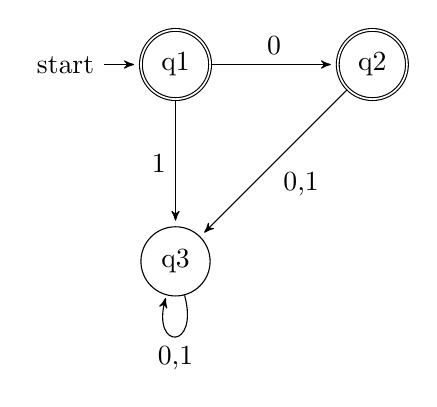
\begin{tikzpicture}[>=stealth',shorten >=2pt, auto, node distance=2.5cm]
    % Nodes {q1, q2, q3, q4, q5, etc}
    \node [state, initial, accepting] 		(q1) 				 {q1};
    \node [state, accepting]                (q2) [right of=q1]	 {q2};
    \node [state] 		                    (q3) [below of=q1]	 {q3};
    
    % Paths
    \path [->] 	(q1) edge 	            node	     {0}	(q2);
    \path [->] 	(q1) edge               node [left]	 {1}	(q3);
    \path [->] 	(q2) edge 	            node	     {0,1}	(q3);
    \path [<->] (q3) edge [loop below]	node	     {0,1}	(q3);
    
    \end{tikzpicture} \\
\end{center}

\noindent
L. \{w$|$ w contains an even number of 0s, or contains exactly two 1s\}
\begin{center}
    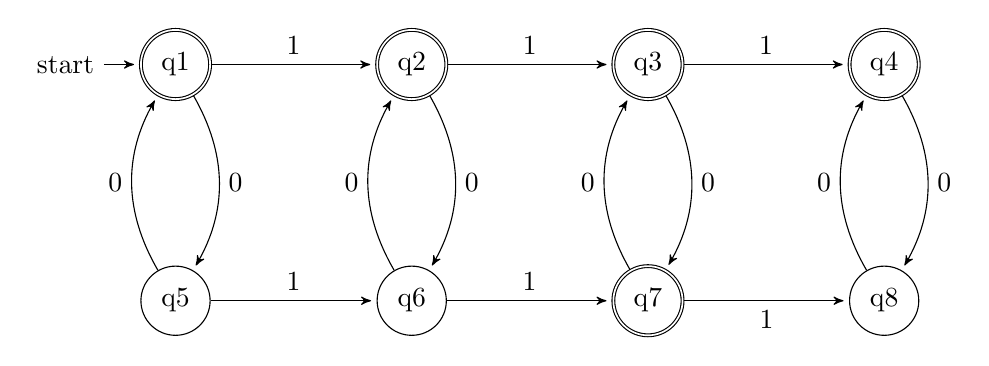
\begin{tikzpicture}[>=stealth',shorten >=2pt, auto, node distance=3
    cm]
    % Nodes {q1, q2, q3, q4, q5, etc}
    \node [state, initial, accepting] 	  (q1) 				   {q1};
    \node [state, accepting] 		      (q2)  [right of=q1]  {q2};
    \node [state, accepting]   	          (q3)  [right of=q2]  {q3};
    \node [state, accepting]	          (q4)  [right of=q3]  {q4};
    \node [state] 	                      (q5)  [below of=q1]  {q5};
    \node [state]                         (q6)  [below of=q2]  {q6};
    \node [state, accepting] 	          (q7)  [below of=q3]  {q7};
    \node [state] 	          		      (q8)  [below of=q4]  {q8};
    
    % Paths
    \path [->] 	(q1) edge	            node	        {1}		(q2);
    \path [->] 	(q2) edge 				node	        {1}		(q3);
    \path [->] 	(q3) edge 				node	        {1}		(q4);

    
    \path [->] 	(q5) edge	            node	        {1}		(q6);
    \path [->] 	(q6) edge 				node	        {1}		(q7);
    \path [->] 	(q7) edge 				node [below]	{1}		(q8);
    
    \path [->] 	(q1) edge [bend left]   node	        {0}		(q5);
    \path [->] 	(q2) edge [bend left]   node	        {0}		(q6);
    \path [->] 	(q3) edge [bend left]   node	        {0}		(q7);
    \path [->] 	(q4) edge [bend left]   node	        {0}		(q8);
    
    \path [->] 	(q5) edge [bend left]   node	        {0}		(q1);
    \path [->] 	(q6) edge [bend left]   node	        {0}		(q2);
    \path [->] 	(q7) edge [bend left]   node	        {0}		(q3);
    \path [->] 	(q8) edge [bend left]   node	        {0}		(q4);
    
    \end{tikzpicture} \\
\end{center}

\noindent
m. The empty set
\begin{center}
    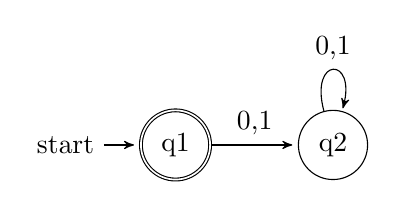
\begin{tikzpicture}[>=stealth',shorten >=2pt, auto, node distance=2cm]
    % Nodes {q1, q2, q3, q4, q5, etc}
    \node [state, initial, accepting] 		(q1) 				 {q1};
    \node [state] 							(q2) [right of=q1]  {q2};
    
    % Paths
    \path [->] 	(q1) edge 				node	{0,1}		(q2);
    \path [->] 	(q2) edge [loop above]	node	{0,1}		(q2);
    
    \end{tikzpicture} \\
\end{center}

\noindent
n. All strings except the empty string
\begin{center}
    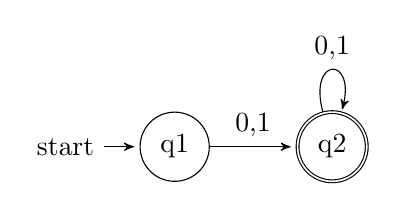
\begin{tikzpicture}[>=stealth',shorten >=2pt, auto, node distance=2cm]
    % Nodes {q1, q2, q3, q4, q5, etc}
    \node [state, initial] 		    (q1) 				 {q1};
    \node [state, accepting] 		(q2) [right of=q1]	 {q2};
    
    % Paths
    \path [->] 	(q1) edge 	            node	{0,1}		(q2);
    \path [->] 	(q2) edge [loop above]	node	{0,1}		(q2);
    
    \end{tikzpicture} \\
\end{center}

%*********************************************************************************
% 1.7 here

\clearpage
\noindent
1.7: b, c, d, e, g, h \\
b. The language of Exercise 1.6l with six states \\
\{w$|$ w contains the substring 0101 (i.e., w = x0101y for some x and y)\}
\begin{center}
    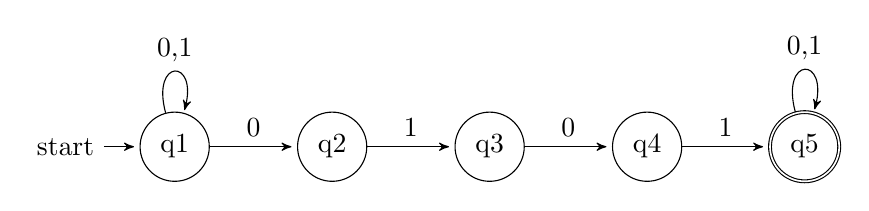
\begin{tikzpicture}[>=stealth',shorten >=2pt, auto, node distance=2cm]
    % Nodes {q1, q2, q3, q4, q5, etc}
    \node [state, initial] 		(q1) 				 {q1};
    \node [state] 				(q2)  [right of=q1]  {q2};
    \node [state]   			(q3)  [right of=q2]  {q3};
    \node [state]   			(q4)  [right of=q3]  {q4};
    \node [state, accepting]	(q5)  [right of=q4]  {q5};
    
    % Paths
    \path [->] 	(q1) edge 				node	{0}		(q2);
    \path [->] 	(q1) edge [loop above] 	node	{0,1}		(q1);
    \path [->] 	(q2) edge 				node	{1}		(q3);
    \path [->] 	(q3) edge 				node	{0}		(q4);
    \path [->] 	(q4) edge 				node	{1}		(q5);
    \path [->] 	(q5) edge [loop above] 	node	{0,1}	(q5);
    
    \end{tikzpicture} \\
\end{center}

\noindent
c. The language of Exercise 1.6l with six states \\
\{w$|$ w contains an even number of 0s, or contains exactly two 1s\}
\begin{center}
    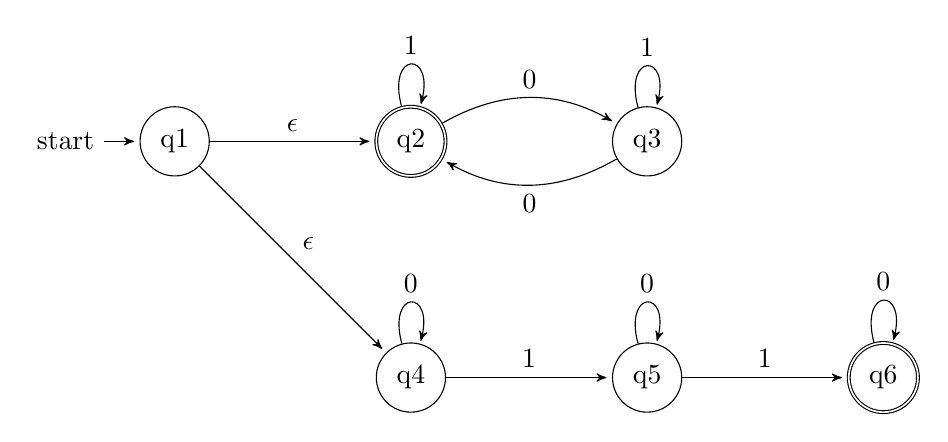
\begin{tikzpicture}[>=stealth',shorten >=2pt, auto, node distance=3cm]
    % Nodes {q1, q2, q3, q4, q5, etc}
    \node [state, initial] 		(q1) 				 {q1};
    \node [state, accepting] 	(q2)  [right of=q1]  {q2};
    \node [state]   			(q3)  [right of=q2]  {q3};
    \node [state]   			(q4)  [below of=q2]  {q4};
    \node [state]   			(q5)  [right of=q4]  {q5};
    \node [state, accepting]	(q6)  [right of=q5]  {q6};
    
    % Paths
    \path [->] 	(q1) edge 				node	{$\epsilon$}		(q2);
    \path [->] 	(q1) edge 				node	{$\epsilon$}		(q4);
    \path [->] 	(q2) edge [loop above] 	node	{1}     (q2);
    \path [->] 	(q2) edge [bend left]	node	{0}		(q3);
    \path [->] 	(q3) edge [bend left]	node	{0}		(q2);
    \path [->] 	(q3) edge [loop above] 	node	{1}     (q3);
    \path [->] 	(q4) edge 				node	{1}		(q5);
    \path [->] 	(q4) edge [loop above] 	node	{0}     (q4);
    \path [->] 	(q5) edge 				node	{1}		(q6);
    \path [->] 	(q5) edge [loop above] 	node	{0}	    (q5);
    \path [->] 	(q6) edge [loop above] 	node	{0}	    (q6);
    
    \end{tikzpicture} \\
\end{center}

\noindent
d. The language {0} with two states
\begin{center}
    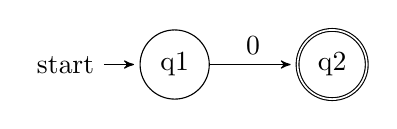
\begin{tikzpicture}[>=stealth',shorten >=2pt, auto, node distance=2cm]
    % Nodes {q1, q2, q3, q4, q5, etc}
    \node [state, initial] 		(q1) 				 {q1};
    \node [state, accepting]	(q2)  [right of=q1]  {q2};
    
    % Paths
    \path [->] 	(q1) edge 				node	{0}		(q2);
    
    \end{tikzpicture} \\
\end{center}

\noindent
e. The language 0*1*0\textsuperscript{+} with three states \\
\begin{center}
    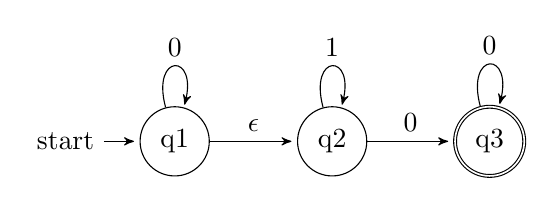
\begin{tikzpicture}[>=stealth',shorten >=2pt, auto, node distance=2cm]
    % Nodes {q1, q2, q3, q4, q5, etc}
    \node [state, initial] 		(q1) 				 {q1};
    \node [state] 		        (q2)  [right of=q1]	 {q2};
    \node [state, accepting]	(q3)  [right of=q2]  {q3};
    
    % Paths
    \path [->] 	(q1) edge 				node	{$\epsilon$}	   (q2);
    \path [->] 	(q1) edge [loop above] 	node	{0}	           (q1);
    \path [->] 	(q2) edge 				node	{0}	           (q3);
    \path [->] 	(q2) edge [loop above] 	node	{1}	           (q2);
    \path [->] 	(q3) edge [loop above] 	node	{0}	           (q3);
    
    \end{tikzpicture} \\
\end{center}

\clearpage
\noindent
g. The language \{$\epsilon$\} with one state \\
\begin{center}
    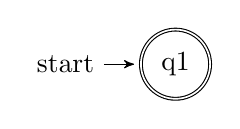
\begin{tikzpicture}[>=stealth',shorten >=2pt, auto, node distance=2cm]
    % Nodes {q1, q2, q3, q4, q5, etc}
    \node [state, initial, accepting] 		(q1) 				 {q1};
    
    % no Paths for this one.
    \end{tikzpicture} \\
\end{center}

\noindent
h. The language 0* with one state \\
\begin{center}
    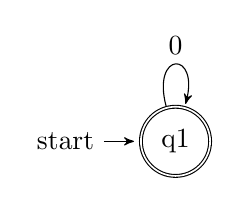
\begin{tikzpicture}[>=stealth',shorten >=2pt, auto, node distance=2cm]
    % Nodes {q1, q2, q3, q4, q5, etc}
    \node [state, initial, accepting] 		(q1) 				 {q1};
    
    % Paths
    \path [->] 	(q1) edge [loop above]	node	{0}		(q1);
    
    \end{tikzpicture} \\
\end{center}

%*********************************************************************************
% 1.8 here

\noindent
1.8: a, b \\
Use the construction in the proof of Theorem 1.45 to give the state \\
diagrams of NFAs recognizing the union of the languages described in \\
1.8 a. Exercise 1.6a
\{w$|$ w begins with a 1 and ends with a 0\}
\begin{center}
	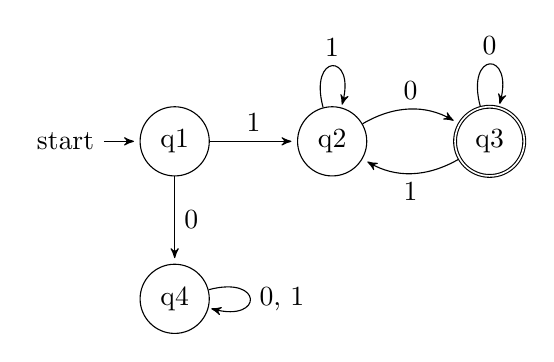
\begin{tikzpicture}[>=stealth',shorten >=2pt, auto, node distance=2cm]
	% Nodes {q1, q2, q3, q4, q5, etc}
	\node [state, initial]    	(q1) 				 {q1};
	\node [state] 				(q2)  [right of=q1]  {q2};
	\node [state, accepting]   	(q3)  [right of=q2]  {q3};
	\node [state]	            (q4)  [below of=q1]  {q4};
	
	% Paths
	\path [->] 	(q1) edge 				node	{1}		(q2);
	\path [->] 	(q1) edge 				node	{0}		(q4);
	\path [->] 	(q2) edge [bend left]	node	{0}		(q3);
	\path [->] 	(q2) edge [loop above] 	node	{1}		(q2);
	\path [->] 	(q3) edge [bend left]	node	{1}		(q2);
	\path [->] 	(q3) edge [loop above] 	node	{0}		(q3);
	\path [->] 	(q4) edge [loop right] 	node	{0, 1}	(q4);
	
	\end{tikzpicture} \\
\end{center}

\noindent
Exercise 1.6b \\
\{w$|$ w contains at least three 1s\}
\begin{center}
	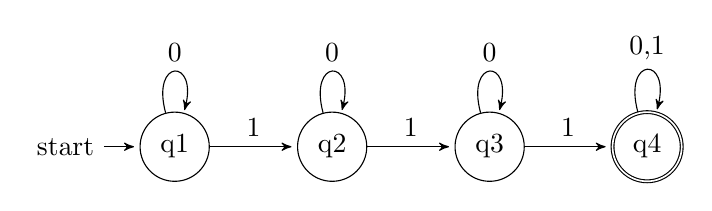
\begin{tikzpicture}[>=stealth',shorten >=2pt, auto, node distance=2cm]
	% Nodes {q1, q2, q3, q4, q5, etc}
	\node [state, initial] 		(q1) 				 {q1};
	\node [state] 				(q2)  [right of=q1]  {q2};
	\node [state]   	        (q3)  [right of=q2]  {q3};
	\node [state, accepting]	(q4)  [right of=q3]  {q4};
	
	% Paths
	\path [->] 	(q1) edge 				node	{1}		(q2);
	\path [->] 	(q1) edge [loop above] 	node	{0}		(q1);
	\path [->] 	(q2) edge 				node	{1}		(q3);
	\path [->] 	(q2) edge [loop above] 	node	{0}		(q2);
	\path [->] 	(q3) edge 				node	{1}		(q4);
	\path [->] 	(q3) edge [loop above] 	node	{0}		(q3);
	\path [->] 	(q4) edge [loop above] 	node	{0,1}	(q4);
	
	\end{tikzpicture} \\
\end{center}

\clearpage
\noindent
Exercise 1.6a and Exercise 1.b joined
\begin{center}
    \begin{tikzpicture}[>=stealth',shorten >=2pt, auto, node distance=3cm]
    % Nodes {q1, q2, q3, q4, q5, etc}
    \node [state, initial] 		(q1) 				 {q1};
    \node [state] 				(q2)  [right of=q1]  {q2};
    \node [state]   			(q3)  [right of=q2]  {q3};
    \node [state, accepting]   	(q4)  [right of=q3]  {q4};
    \node [state]   			(q5)  [below of=q2]  {q5};
    \node [state]   			(q6)  [right of=q5]  {q6};
    \node [state]   			(q7)  [right of=q6]  {q7};
    \node [state, accepting]	(q8)  [right of=q7]  {q8};
    
    % Paths
    \path [->] 	(q1) edge 				node	{$\epsilon$}	(q2);
    \path [->] 	(q1) edge 				node	{$\epsilon$}	(q5);
    \path [->] 	(q2) edge				node	{1}				(q3);
    \path [->] 	(q3) edge [loop above] 	node	{0,1}     		(q3);
	\path [->] 	(q3) edge				node	{0}				(q4);
    \path [->] 	(q5) edge 				node	{1}				(q6);
    \path [->] 	(q5) edge [loop above] 	node	{0}	    		(q5);
    \path [->] 	(q6) edge 				node	{1}				(q7);
    \path [->] 	(q6) edge [loop above] 	node	{0}	    		(q6);
    \path [->] 	(q7) edge 				node	{1}				(q8);
    \path [->] 	(q7) edge [loop above] 	node	{0}	    		(q7);
    \path [->] 	(q8) edge [loop above] 	node	{0,1}	    	(q8);
    
    \end{tikzpicture} \\
\end{center}

\noindent
1.8 b. Exercises 1.6c and 1.6f \\
Exercises 1.6c
\begin{center}
	\begin{tikzpicture}[>=stealth',shorten >=2pt, auto, node distance=3cm]
	% Nodes {q1, q2, q3, q4, q5, etc}
	\node [state, initial] 		(q1) 				 {q1};
	\node [state] 				(q2)  [right of=q1]  {q2};
	\node [state]   	        (q3)  [right of=q2]  {q3};
	\node [state]   	        (q4)  [right of=q3]  {q4};
	\node [state, accepting]	(q5)  [right of=q4]  {q5};
	
	% Paths
	\path [->] 	(q1) edge 				node	{0}		(q2);
	\path [->] 	(q1) edge [loop above] 	node	{1}		(q1);
	\path [->] 	(q2) edge 				node	{1}		(q3);
	\path [->] 	(q2) edge [loop above] 	node	{0}		(q2);
	\path [->] 	(q3) edge 				node	{0}		(q4);
	\path [->] 	(q3) edge [bend left]	node	{1}		(q1);
	\path [->] 	(q4) edge 				node	{1}		(q5);
	\path [->] 	(q4) edge [bend left] 	node	{0}	    (q2);
	\path [->] 	(q5) edge [loop above] 	node	{0,1}		(q5);
	
	\end{tikzpicture} \\
\end{center}

\noindent
Exercises 1.6f
\begin{center}
	\begin{tikzpicture}[>=stealth',shorten >=2pt, auto, node distance=2cm]
	% Nodes {q1, q2, q3, q4, q5, etc}
	\node [state, initial, accepting] 		(q1) 				 {q1};
	\node [state, accepting] 				(q2)  [right of=q1]  {q2};
	\node [state, accepting]   	            (q3)  [right of=q2]  {q3};
	\node [state]	                        (q4)  [right of=q3]  {q4};
	
	% Paths
	\path [->] 	(q1) edge [bend left]	node	{1}		(q2);
	\path [->] 	(q1) edge [loop above] 	node	{0}		(q1);
	\path [->] 	(q2) edge [bend left]	node	{0}		(q1);
	\path [->] 	(q2) edge 				node	{1}		(q3);
	\path [->] 	(q3) edge 				node	{0}		(q4);
	\path [->] 	(q3) edge [loop above] 	node	{1}		(q3);
	\path [->] 	(q4) edge [loop above] 	node	{0,1}	(q4);
	
	\end{tikzpicture} \\
\end{center}

\clearpage
\noindent
Exercises 1.6c and Exercises 1.6f joined
\begin{center}
	\begin{tikzpicture}[>=stealth',shorten >=2pt, auto, node distance=2cm]
	% Nodes {q1, q2, q3, q4, q5, etc}
	\node [state, initial] 		(q1) 				  {q1};
	\node [state] 				(q2)   [right of=q1]  {q2};
	\node [state]   	        (q3)   [right of=q2]  {q3};
	\node [state]   	        (q4)   [right of=q3]  {q4};
	\node [state]   	        (q5)   [right of=q4]  {q5};
	\node [state, accepting]	(q6)   [right of=q5]  {q6};
	\node [state, accepting]	(q7)   [below of=q2]  {q7};
	\node [state, accepting]	(q8)   [right of=q7]  {q8};
	\node [state, accepting]	(q9)   [right of=q8]  {q9};
	\node [state]				(q10)  [right of=q9]  {q10};
	
	% Paths
	\path [->] 	(q1) edge 				node	{$\epsilon$}		(q2);
	\path [->] 	(q1) edge 				node	{$\epsilon$}		(q7);
	\path [->] 	(q2) edge 				node	{0}					(q3);
	\path [->] 	(q2) edge [loop above] 	node	{0,1}				(q2);
	\path [->] 	(q3) edge 				node	{1}					(q4);
	\path [->] 	(q4) edge 				node	{0}					(q5);
	\path [->] 	(q5) edge 				node	{1}					(q6);
	\path [->] 	(q6) edge [loop above] 	node	{0,1}				(q6);
	
	\path [->] 	(q7) edge 					node			{1}		(q8);
	\path [->] 	(q7) edge  [loop below] 	node			{0}		(q7);
	\path [->] 	(q8) edge 					node			{1}		(q9);
	\path [->] 	(q8) edge  [loop below] 	node			{0}		(q8);
	\path [->] 	(q9) edge 					node [below]	{0}		(q10);
	\path [->] 	(q9) edge  [loop below] 	node			{1}		(q9);
	\path [->] 	(q10) edge [bend right]		node [above]	{1}		(q9);
	\path [->] 	(q10) edge [loop below] 	node			{0}		(q10);
	
	\end{tikzpicture} \\
\end{center}

%*********************************************************************************
% 1.9 here

\noindent
1.9: a, b \\
Use the construction in the proof of Theorem 1.47 to give the state diagrams \\
of NFAs recognizing the concatenation of the languages described in \\
a. Exercises 1.6g and 1.6i \\
Exercise 1.6g
\begin{center}
    \begin{tikzpicture}[>=stealth',shorten >=2pt, auto, node distance=2cm]
    % Nodes {q1, q2, q3, q4, q5, etc}
    \node [state, initial, accepting] 	(q1) 				 {q1};
    \node [state, accepting] 			(q2)  [right of=q1]  {q2};
    \node [state, accepting]   	        (q3)  [right of=q2]  {q3};
    \node [state, accepting]	        (q4)  [right of=q3]  {q4};
    \node [state, accepting] 			(q5)  [right of=q4]  {q5};
    \node [state] 			            (q6)  [right of=q5]  {q6};
    
    % Paths
    \path [->] 	(q1) edge	            node			{0,1}	(q2);
    \path [->] 	(q2) edge 				node			{0,1}	(q3);
    \path [->] 	(q3) edge 				node			{0,1}	(q4);
    \path [->] 	(q4) edge               node        	{0,1}	(q5);
    \path [->] 	(q5) edge            	node			{0,1}	(q6);
    
    \end{tikzpicture} \\
\end{center}

\noindent
Exercise 1.6i \\
\{w$|$ every odd position of w is a 1\}
\begin{center}
	\begin{tikzpicture}[>=stealth',shorten >=2pt, auto, node distance=2.5cm]
	% Nodes {q1, q2, q3, q4, q5, etc}
	\node [state, initial] 		(q1) 				 {q1};
	\node [state] 		        (q2) [right of=q1]	 {q2};
	\node [state, accepting] 	(q3) [below of=q1]	 {q3};
	\node [state, accepting] 	(q4) [right of=q3]	 {q4};
	
	% Paths
	\path [->] 	(q1) edge 	            node	     {0}		(q2);
	\path [->] 	(q1) edge  				node [left]	 {1}		(q3);
	\path [->] 	(q2) edge [loop above]	node	     {0,1}	    (q2);
	\path [->] 	(q3) edge [bend left]   node	     {0,1}		(q4);
	\path [->] 	(q4) edge [bend left]   node	     {1}		(q3);
	\path [->] 	(q4) edge 	            node	     {0}		(q2);
	
	\end{tikzpicture} \\
\end{center}

\clearpage
\noindent
Exercise 1.6g and Exercise 1.6i joined
\begin{center}
    \begin{tikzpicture}[>=stealth',shorten >=2pt, auto, node distance=2cm]
    % Nodes {q1, q2, q3, q4, q5, etc}
    \node [state, initial] 	    (q1) 				 {q1};
    \node [state] 			    (q2)  [right of=q1]  {q2};
    \node [state]   	        (q3)  [right of=q2]  {q3};
    \node [state]	            (q4)  [right of=q3]  {q4};
    \node [state] 			    (q5)  [right of=q4]  {q5};
    \node [state] 			    (q6)  [right of=q5]  {q6};
    \node [state, accepting] 	(q7)  [below of=q3]  {q7};
    \node [state, accepting] 	(q8)  [below of=q7]  {q8};
    
    % Paths
    \path [->] 	(q1) edge	            node			{0,1}	(q2);
    \path [->] 	(q2) edge 				node			{0,1}	(q3);
    \path [->] 	(q3) edge 				node			{0,1}	(q4);
    \path [->] 	(q4) edge               node        	{0,1}	(q5);
    \path [->] 	(q5) edge            	node			{0,1}	(q6);
    
    \path [->] 	(q1) edge	            node  [below]	{$\epsilon$}	(q7);
    \path [->] 	(q2) edge	            node  [below]	{$\epsilon$}	(q7);
    \path [->] 	(q3) edge	            node  [left]	{$\epsilon$}	(q7);
    \path [->] 	(q4) edge	            node  [below]	{$\epsilon$}	(q7);
    \path [->] 	(q5) edge	            node  [below]	{$\epsilon$}	(q7);
    \path [->] 	(q6) edge	            node  [below]	{$\epsilon$}	(q7);
    \path [->] 	(q7) edge            	node			{1}				(q8);
    \path [->] 	(q8) edge [bend left]   node  			{$\epsilon$}	(q7);
    
    \end{tikzpicture} \\
\end{center}

\noindent
b. Exercises 1.6b and 1.6m \\
Exercise 1.6b \\
\{w$|$ w contains at least three 1s\}
\begin{center}
	\begin{tikzpicture}[>=stealth',shorten >=2pt, auto, node distance=2cm]
	% Nodes {q1, q2, q3, q4, q5, etc}
	\node [state, initial] 		(q1) 				 {q1};
	\node [state] 				(q2)  [right of=q1]  {q2};
	\node [state]   	        (q3)  [right of=q2]  {q3};
	\node [state, accepting]	(q4)  [right of=q3]  {q4};
	
	% Paths
	\path [->] 	(q1) edge 				node	{1}		(q2);
	\path [->] 	(q1) edge [loop above] 	node	{0}		(q1);
	\path [->] 	(q2) edge 				node	{1}		(q3);
	\path [->] 	(q2) edge [loop above] 	node	{0}		(q2);
	\path [->] 	(q3) edge 				node	{1}		(q4);
	\path [->] 	(q3) edge [loop above] 	node	{0}		(q3);
	\path [->] 	(q4) edge [loop above] 	node	{0,1}	(q4);
	
	\end{tikzpicture} \\
\end{center}

\noindent
Exercise 1.6m - The empty set
\begin{center}
	\begin{tikzpicture}[>=stealth',shorten >=2pt, auto, node distance=2cm]
	% Nodes {q1, q2, q3, q4, q5, etc}
	\node [state, initial, accepting] 		(q1) 				 {q1};
	\node [state] 							(q2) [right of=q1]  {q2};
	
	% Paths
	\path [->] 	(q1) edge 				node	{0,1}		(q2);
	\path [->] 	(q2) edge [loop above]	node	{0,1}		(q2);
	
	\end{tikzpicture} \\
\end{center}

\noindent
Exercises 1.6b and 1.6m joined \\
\begin{center}
	\begin{tikzpicture}[>=stealth',shorten >=2pt, auto, node distance=2cm]
	% Nodes {q1, q2, q3, q4, q5, etc}
	\node [state, initial] 		(q1) 				 {q1};
	\node [state] 				(q2)  [right of=q1]  {q2};
	\node [state]   	        (q3)  [right of=q2]  {q3};
	\node [state]				(q4)  [right of=q3]  {q4};
	\node [state]				(q5)  [right of=q4]  {q5};
	
	% Paths
	\path [->] 	(q1) edge 				node	{1}				(q2);
	\path [->] 	(q1) edge [loop above] 	node	{0,1}			(q1);
	\path [->] 	(q2) edge 				node	{1}				(q3);
	\path [->] 	(q2) edge [loop above] 	node	{0,1}			(q2);
	\path [->] 	(q3) edge 				node	{1}				(q4);
	\path [->] 	(q3) edge [loop above] 	node	{0,1}			(q3);
	\path [->] 	(q4) edge [loop above] 	node	{0,1}			(q4);
	\path [->] 	(q4) edge 				node	{$\epsilon$}	(q5);
	
	\end{tikzpicture} \\
\end{center}

%*********************************************************************************
% 1.10 here

\clearpage
\noindent
1.10: a, b, c \\
Use the construction in the proof of Theorem 1.49 to give the state \\
diagrams of NFAs recognizing the star of the languages described in \\

\noindent
a. Exercise 1.6b \\
\{w$|$ w contains at least three 1s\}
\begin{center}
	\begin{tikzpicture}[>=stealth',shorten >=2pt, auto, node distance=2cm]
	% Nodes {q1, q2, q3, q4, q5, etc}
	\node [state, initial] 		(q1) 				 {q1};
	\node [state] 				(q2)  [right of=q1]  {q2};
	\node [state]   	        (q3)  [right of=q2]  {q3};
	\node [state, accepting]	(q4)  [right of=q3]  {q4};
	
	% Paths
	\path [->] 	(q1) edge 				node	{1}		(q2);
	\path [->] 	(q1) edge [loop above] 	node	{0}		(q1);
	\path [->] 	(q2) edge 				node	{1}		(q3);
	\path [->] 	(q2) edge [loop above] 	node	{0}		(q2);
	\path [->] 	(q3) edge 				node	{1}		(q4);
	\path [->] 	(q3) edge [loop above] 	node	{0}		(q3);
	\path [->] 	(q4) edge [loop above] 	node	{0,1}	(q4);
	
	\end{tikzpicture} \\
\end{center}

\noindent
b. Exercise 1.6j \\
\{w$|$ w contains at least two 0s and at most one 1\}
\begin{center}
	\begin{tikzpicture}[>=stealth',shorten >=2pt, auto, node distance=2cm]
	% Row 1
	\node [state, initial] 		(q1) 				 {q1};
	\node [state] 				(q2)  [right of=q1]  {q2};
	\node [state]   			(q3)  [right of=q2]  {q3};
	\node [state]   			(q4)  [right of=q3]  {q4};
	\node [state]   			(q5)  [right of=q4]  {q5};
	\node [state, accepting]   	(q6)  [right of=q5]  {q6};
	
	% Row 2
	\node [state] 	            (q7)   [below of=q2]  {q7};
	\node [state]   			(q8)   [right of=q7]  {q8};
	\node [state]   			(q9)   [right of=q8]  {q9};
	\node [state]   			(q10)  [right of=q9]  {q10};
	
	% Row 3
	\node [state] 	            (q11)  [below of=q7]   {q11};
	\node [state]   			(q12)  [right of=q11]  {q12};
	\node [state]   			(q13)  [right of=q12]  {q13};
	\node [state]   			(q14)  [right of=q13]  {q14};
	
	% Row 4
	\node [state] 	            (q15)  [below of=q11]  {q15};
	\node [state]   			(q16)  [right of=q15]  {q16};
	\node [state]   			(q17)  [right of=q16]  {q17};
	\node [state]   			(q18)  [right of=q17]  {q18};
	
	% First Column
	\path [->] 	(q1) edge  [loop above]   	node	{0}					(q1);
	\path [->] 	(q1) edge	            	node	{$\epsilon$}		(q2);
	\path [->] 	(q1) edge	            	node	{$\epsilon$}		(q7);
	\path [->] 	(q1) edge	            	node	{$\epsilon$}		(q11);
	\path [->] 	(q1) edge	            	node	{$\epsilon$}		(q15);
	
	% 2nd Column
	\path [->] 	(q2)  edge	           	 	node	{0}					(q3);
	\path [->] 	(q7)  edge	            	node	{0}					(q8);
	\path [->] 	(q11) edge	            	node	{0}					(q12);
	\path [->] 	(q15) edge	            	node	{1}					(q16);
	
	% 3rd Column
	\path [->] 	(q3)  edge	           	 	node	{0}					(q4);
	\path [->] 	(q8)  edge	            	node	{1}					(q9);
	\path [->] 	(q12) edge	            	node	{0}					(q13);
	\path [->] 	(q16) edge	            	node	{0}					(q17);
	
	% 4th Column
	\path [->] 	(q4)  edge	           	 	node	{0}					(q5);
	\path [->] 	(q9)  edge	            	node	{0}					(q10);
	\path [->] 	(q13) edge	            	node	{1}					(q14);
	\path [->] 	(q17) edge	            	node	{0}					(q18);
	
	% Last Column
	\path [->] 	(q6)  edge  [loop above]   	node	{0}					(q6);
	\path [->] 	(q5)  edge	            	node	{$\epsilon$}		(q6);
	\path [->] 	(q10) edge	            	node	{$\epsilon$}		(q6);
	\path [->] 	(q14) edge	            	node	{$\epsilon$}		(q6);
	\path [->] 	(q18) edge	            	node	{$\epsilon$}		(q6);
	
	\end{tikzpicture} \\
\end{center}

\noindent
c. Exercise 1.6m \\
\begin{center}
	\begin{tikzpicture}[>=stealth',shorten >=2pt, auto, node distance=2cm]
	% Nodes {q1, q2, q3, q4, q5, etc}
	\node [state, initial, accepting] 		(q1) 				 {q1};
	\node [state] 							(q2) [right of=q1]   {q2};
	
	% Paths
	\path [->] 	(q1) edge 				node	{$\epsilon$}	(q2);
	
	\end{tikzpicture} \\
\end{center}

%*********************************************************************************
% 1.12 here

\noindent
1.12 \\
Let D = \{w$|$ w contains an even number of a$\textsc{\char13}$s and an odd number of 
b$\textsc{\char13}$s  \\
and does not contain the substring ab\}. Give a DFA with five states that \\
recognizes D and a regular expression that generates D. \\
(Suggestion: Describe D more simply.) \\

\begin{center}
	\begin{tikzpicture}[>=stealth',shorten >=2pt, auto, node distance=3cm]
	% Nodes {q1, q2, q3, q4, q5, etc}
	\node [state, initial] 		(q1) 				 {q1};
	\node [state, accepting] 	(q2)  [right of=q1]  {q2};
	\node [state]   	        (q3)  [right of=q2]  {q3};
	\node [state, accepting]	(q4)  [right of=q3]  {q4};
	\node [state]				(q5)  [below of=q3]  {q5};
	
	% Paths
	\path [->] 	(q1) edge [bend left]	node	{b}				(q2);
	\path [->] 	(q1) edge [bend right]	node	{a}				(q5);
	\path [->] 	(q2) edge [bend left] 	node	{b}				(q1);
	\path [->]  (q2) edge 				node	{a}				(q3);
	\path [->] 	(q3) edge [bend left]	node	{a}				(q4);
	\path [->]  (q3) edge 				node	{b}				(q5);
	\path [->] 	(q4) edge [bend left] 	node	{a}				(q3);
	\path [->]  (q4) edge 				node	{b}				(q5);
	\path [->] 	(q5) edge [loop below]	node	{a,b}			(q5);
	
	\end{tikzpicture} \\
\end{center}

\noindent
R1 = \{w$|$ w contains an even number of a$\textsc{\char13}$s\} \\
R1 = (aa)* \\

\noindent
R2 =  \{w$|$ w contains an odd number of b$\textsc{\char13}$s and does not contain the \\
substring ab \} \\
R2 = b(bb)* \\

\noindent
R = b(bb)*(aa)* \\

%*********************************************************************************
% 1.13 here

\clearpage
\noindent
1.13 \\
\noindent
Let F be the language of all strings over {0,1} that do not contain a pair of 1s that
are separated by an odd number of symbols. Give the state diagram of a DFA with
five states that recognizes F.
\begin{center}
	\begin{tikzpicture}[>=stealth',shorten >=2pt, auto, node distance=3cm]
	% Nodes {q1, q2, q3, q4, q5, etc}
	\node [state, initial, accepting] 		(q1) 				 {q1};
	\node [state, accepting] 				(q2)  [right of=q1]  {q2};
	\node [state, accepting]   	        	(q3)  [right of=q2]  {q3};
	\node [state, accepting]				(q4)  [below of=q2]  {q4};
	\node [state]							(q5)  [below of=q3]  {q5};
	
	% Paths
	\path [->] 	(q1) edge 				node	{1}				(q2);
	\path [->] 	(q1) edge [loop above]	node	{0}				(q1);
	\path [->] 	(q2) edge 				node	{1}				(q3);
	\path [->] 	(q2) edge [bend left]	node	{0}				(q4);
	\path [->] 	(q3) edge				node	{1}				(q5);
	\path [->] 	(q3) edge [loop above]	node	{0}				(q3);
	\path [->] 	(q4) edge [bend left]	node	{0}				(q2);
	\path [->] 	(q4) edge				node	{1}				(q5);
	\path [->] 	(q5) edge [loop right]	node	{0,1}			(q5);
	
	\end{tikzpicture} \\
\end{center}

%*********************************************************************************
% 1.16 here

\noindent
1.16 a. \\
\begin{center}
    \begin{tikzpicture}[>=stealth',shorten >=2pt, auto, node distance=2cm]
    % Nodes {q1, q2, q3, q4, q5, etc}
    \node [state] 						(q1) 				 {q1};
    \node [state] 						(q2)  [right of=q1]  {q2};
    \node [state, initial, initial where=above, accepting]   (q3)  [right of=q2]  {q3};
    \node [state, accepting]   			(q4)  [right of=q3]  {q4};
    
    % Paths
    \path [->] 	(q1) edge [loop above] 	node	{a,b}	(q1);
    \path [->] 	(q2) edge 				node	{a}		(q1);
    \path [->] 	(q2) edge [bend left]	node	{b}		(q3);
    \path [->] 	(q3) edge [bend left]	node	{b}		(q2);
    
    \path [->] 	(q3) edge 				node	{a}		(q4);
    \path [->] 	(q4) edge [loop above] 	node	{a,b}	(q4);
    
    \end{tikzpicture} \\
\end{center}

\noindent
b.
\begin{center}
    \begin{tikzpicture}[>=stealth',shorten >=2pt, auto, node distance=2cm]
    % Nodes {q1, q2, q3, q4, q5, etc}
    \node [state,  initial, accepting] 	(q1) 				 {q1};
    \node [state, accepting] 			(q2)  [right of=q1]  {q2};
    \node [state, accepting]   			(q3)  [right of=q2]  {q3};
    \node [state]   					(q4)  [below of=q1]  {q4};
    
    % Paths
    \path [->] 	(q1) edge 				node	{a}		(q4);
    \path [->] 	(q1) edge [bend left] 	node	{a}		(q3);
    \path [->] 	(q2) edge 				node	{a}		(q1);
    \path [->] 	(q2) edge [loop below] 	node	{b}		(q2);
    \path [->] 	(q3) edge 				node	{b}		(q2);
    \path [->] 	(q3) edge [loop below] 	node	{a}		(q3);
    \path [->] 	(q4) edge [loop left] 	node	{a,b}	(q4);
    
    \end{tikzpicture} \\
\end{center}

%*********************************************************************************
% 1.17 here

\clearpage
\noindent
1.17: a, b

\noindent
a. Give an NFA recognizing the language  $(01 \bigcup 001 \bigcup 010)\textsuperscript{*}$.
\begin{center}
	\begin{tikzpicture}[>=stealth',shorten >=2pt, auto, node distance=2cm]
	% Row 1
	\node [state, initial, accepting] 		(q0) 				 	{q0};
	\node [state] 							(q1)  [right of=q0]	 	{q1};
	\node [state] 							(q2)  [right of=q1]  	{q2};
	\node [state]   						(q3)  [right of=q2]  	{q3};
	\node [state]   						(q4)  [right of=q3]  	{q4};
	\node [state, accepting]   				(q5)  [right of=q4]  	{q5};
	
	% Row 2
	\node [state] 	            (q7)   [below of=q2]  	{q7};
	\node [state]   			(q8)   [right of=q7]  	{q8};
	\node [state]   			(q9)   [right of=q8]  	{q9};
	\node [state]   			(q10)  [right of=q9]  	{q10};
	\node [state] 				(q15)  [right of=q10] 	{q15};
	\node [state, accepting] 	(q16)  [right of=q15] 	{q16};
	
	% Row 3
	\node [state] 	            (q11)  [below of=q7]   	{q11};
	\node [state]   			(q12)  [right of=q11]  	{q12};
	\node [state]   			(q13)  [right of=q12]  	{q13};
	\node [state]   			(q14)  [right of=q13]  	{q14};
	\node [state] 				(q17)  [right of=q14] 	{q17};
	\node [state, accepting] 	(q18)  [right of=q17] 	{q18};
	
	% First Column
	\path [->] 	(q0) edge	            	node	{$\epsilon$}		(q1);
	
	% 2nd Column
	\path [->] 	(q1) edge	            	node	{$\epsilon$}		(q2);
	\path [->] 	(q1) edge	            	node	{$\epsilon$}		(q7);
	\path [->] 	(q1) edge	            	node	{$\epsilon$}		(q11);
	
	% 3rd Column
	\path [->] 	(q2)  edge	           	 	node	{0}					(q3);
	\path [->] 	(q7)  edge	            	node	{0}					(q8);
	\path [->] 	(q11) edge	            	node	{0}					(q12);
	
	% 4th Column
	\path [->] 	(q3)  edge	           	 	node	{$\epsilon$}		(q4);
	\path [->] 	(q8)  edge	            	node	{$\epsilon$}		(q9);
	\path [->] 	(q12) edge	            	node	{$\epsilon$}		(q13);
	
	% 5th Column
	\path [->] 	(q4)  edge	           	 	node	{1}					(q5);
	\path [->] 	(q9)  edge	            	node	{0}					(q10);
	\path [->] 	(q13) edge	            	node	{1}					(q14);
	\path [->] 	(q5)  edge	[bend right, out=-90, in=-90, looseness=.5]	node	{$\epsilon$}		(q1);
	
	% 6th Column
	\path [->] 	(q10)  edge	           	 	node	{$\epsilon$}		(q15);
	\path [->] 	(q14)  edge	            	node	{$\epsilon$}		(q17);
	
	% 7th Column
	\path [->] 	(q15)  edge	           	 	node	{1}					(q16);
	\path [->] 	(q17)  edge	            	node	{0}					(q18);
	\path [->] 	(q16)  edge	[bend right, out=-90, in=-90, looseness=1]	node	{$\epsilon$}		(q1);
	\path [->] 	(q18)  edge	[bend left, out=90, in=90, looseness=1.1] 	node	{$\epsilon$}		(q1);
	
	\end{tikzpicture} \\
\end{center}

\clearpage
\noindent
b. Convert this NFA to an equivalent DFA. Give only the portion of the \\
DFA that is reachable from the start state.
\begin{center}
	\begin{tikzpicture}[>=stealth',shorten >=2pt, auto, node distance=3cm]
	% Nodes {q1, q2, q3, q4, q5, etc}
	\node [state,  initial, accepting] 	(q1) 				 {q1};
	\node [state] 						(q2)  [right of=q1]  {q2};
	\node [state, accepting]   			(q3)  [right of=q2]  {q3};
	\node [state, accepting]   			(q4)  [right of=q3]  {q4};
	\node [state] 						(q5)  [below of=q2]  {q5};
	
	% Paths
	\path [->] 	(q1) edge 				node			{0}		(q2);
	\path [->] 	(q1) edge [loop below] 	node			{1}		(q1);
	\path [->] 	(q2) edge 				node			{0}		(q5);
	\path [->] 	(q3) edge [bend right] 	node [above]	{0,1}	(q1);
	\path [->] 	(q2) edge 				node			{1}		(q3);
	\path [->] 	(q3) edge 				node			{0}		(q4);
	\path [->] 	(q4) edge [bend right, out=-90, in=-90, looseness=.5] 	node [above]	{0,1}	(q1);
	\path [->] 	(q5) edge 				node			{1}		(q4);
	
	\end{tikzpicture} \\
\end{center}

%*********************************************************************************
% 1.18 here

\noindent
1.18 a. \{w$|$ w begins with a 1 and ends with a 0\}
\begin{center} $1\sum\textsuperscript{*}0$ \end{center}

\noindent
b. \{w$|$ w contains at least three 1s\}
\begin{center} 
$\sum\textsuperscript{*}1\sum\textsuperscript{*}1\sum\textsuperscript{*}1\sum\textsuperscript{*}$ 
\end{center}

\noindent
c. \{w$|$ w contains the substring 0101 (i.e., w = x0101y for some x and y)\}
\begin{center} $\sum\textsuperscript{*}0101\sum\textsuperscript{*}$ \end{center}

\noindent
d. \{w$|$ w has length at least 3 and its third symbol is a 0\}
\begin{center} $\sum\sum0\sum\textsuperscript{*}$ \end{center}

\noindent
e. \{w$|$ w starts with 0 and has odd length, or starts with 1 and has even length\}
\begin{center} $(0\bigcup1\sum)(\sum\sum)\textsuperscript{*}$ \end{center}

\noindent
f. \{w$|$ w doesn’t contain the substring 110\}
\begin{center} $0\textsuperscript{*}(10\textsuperscript{+})\textsuperscript{*}1\textsuperscript{*}$
\end{center}

\clearpage
\noindent
g. \{w$|$ the length of w is at most 5\}
\begin{center} $(\epsilon\bigcup\sum)\textsuperscript{5}$ \end{center}

\noindent
h. \{w$|$ w is any string except 11 and 111\} 
\begin{center} 
$\epsilon \bigcup \sum \bigcup 0 \sum \bigcup 10 \bigcup 0 \sum\sum \bigcup 10\sum \bigcup 110 \bigcup \sum \textsuperscript{3} \sum \textsuperscript{+} $
\end{center}

\noindent
I. \{w$|$ every odd position of w is a 1\}
\begin{center} 
$(1 \sum) \textsuperscript{*}(\epsilon \bigcup 1) $
\end{center}

\noindent
j. \{w$|$ w contains at least two 0s and at most one 1\}
\begin{center} 
$00 \textsuperscript{+} \bigcup 100 \textsuperscript{+} \bigcup 0 \textsuperscript{+}
 10 \textsuperscript{+} \bigcup 00 \textsuperscript{+} 1 $
\end{center}

\noindent
k. \{", 0\}
\begin{center} $ 0 \bigcup \epsilon $ \end{center}

\noindent
L. \{w$|$ w contains an even number of 0s, or contains exactly two 1s\}
\begin{center}
$ 1 \textsuperscript{*} (01\textsuperscript{*}01\textsuperscript{*}) \bigcup 0 
     \textsuperscript{*} 10 \textsuperscript{*} 10 \textsuperscript{*} $
\end{center}

\noindent
m. The empty set
\begin{center} $ \emptyset $ \end{center}

\noindent
n. All strings except the empty string
\begin{center} $ \sum \textsuperscript{+} $ \end{center}

%*********************************************************************************
% 1.20 here

\noindent
1.20: a, b, c, d, e, f, g, h \\
\noindent
a. Members: ab, abb \\
Not members: ba, bba \\

\noindent
b. Members: ab, ababab \\
Not members: aba, bab \\

\noindent
c. Members: aaa, bbb \\
Not members: aabb, bbaa \\

\noindent
d. Members: aaa, aaaaaa  \\
Not members: a, aaaa \\

\noindent
e. Members: aba, bbaaabaabb \\
Not members: a, b \\

\noindent
f. Members: aba, bab \\
Not members: ababab, ba \\

\noindent
g. Members: b, ab \\
Not members: a, ba \\

\noindent
h. Members: a, bbab \\
Not members: b, $\epsilon$ \\

%*********************************************************************************
% 1.21 here

\noindent
1.21 a.
\begin{center}
    \begin{tikzpicture}[>=stealth',shorten >=2pt, auto, node distance=3cm]
    % Nodes {q1, q2, q3, q4, q5, etc}
    \node [state, initial] 		(q1) 				 {q1};
    \node [state] 				(q2)  [right of=q1]  {q2};
    \node [state]   	        (q3)  [right of=q2]  {q3};
    \node [state, accepting]	(q4)  [right of=q3]  {q4};
    
    % Paths
    \path [->] 	(q1) edge 				node	{$\epsilon$}	(q2);
    \path [->] 	(q2) edge [bend left]	node	{b}				(q3);
    \path [->] 	(q2) edge [loop above] 	node	{a}				(q2);
    \path [->] 	(q3) edge [bend left] 	node	{b}				(q2);
    \path [->] 	(q3) edge [loop above] 	node	{a}				(q3);
    \path [->] 	(q3) edge 				node	{$\epsilon$}	(q4);
    
    \end{tikzpicture} \\
\end{center}

\begin{center}
	\begin{tikzpicture}[>=stealth',shorten >=2pt, auto, node distance=3cm]
	% Nodes {q1, q2, q3, q4, q5, etc}
	\node [state, initial] 		(q1) 				 {q1};
	\node [state] 				(q2)  [right of=q1]  {q2};
	\node [state, accepting]	(q3)  [right of=q2]  {q3};
	
	% Paths
	\path [->] 	(q1) edge 				node	{$\epsilon$}	(q2);
	\path [->] 	(q2) edge				node	{ba*}			(q3);
	\path [->] 	(q2) edge [loop above] 	node	{a $\bigcup$ ba*b}				(q2);
	
	\end{tikzpicture} \\
\end{center}

\begin{center}
	\begin{tikzpicture}[>=stealth',shorten >=2pt, auto, node distance=4cm]
	% Nodes {q1, q2, q3, q4, q5, etc}
	\node [state, initial] 		(q1) 				 {q1};
	\node [state, accepting]	(q2)  [right of=q1]  {q2};
	
	% Paths
	\path [->] 	(q1) edge 	[bend left]	node	{(a $\bigcup$ ba*b)*ba*}	(q2);
	
	\end{tikzpicture} \\
\end{center}

\clearpage
b.
\begin{center}
	\begin{tikzpicture}[>=stealth',shorten >=2pt, auto, node distance=3cm]
	% Nodes {q1, q2, q3, q4, q5, etc}
	\node [state, initial] 		(q1) 				 {q1};
	\node [state] 				(q2)  [right of=q1]  {q2};
	\node [state]   	        (q3)  [right of=q2]  {q3};
	\node [state, accepting]	(q4)  [below of=q2]  {q4};
	\node [state]   	        (q5)  [right of=q4]  {q5};	
	
	% Paths
	\path [->] 	(q1) edge 					node	{$\epsilon$}		(q2);
	\path [->] 	(q2) edge 	[bend left]		node	{a $\bigcup$ b}		(q3);
	\path [->] 	(q2) edge 					node	{$\epsilon$}		(q4);
	\path [->] 	(q3) edge 	[loop right]	node	{a}					(q3);
	\path [->] 	(q3) edge 	[bend left]		node	{b}					(q5);
	\path [->] 	(q5) edge 					node	{$\epsilon$}		(q4);
	\path [->] 	(q5) edge 	[bend left]		node	{a}					(q2);
	\path [->] 	(q5) edge 	[bend left]		node	{b}					(q3);
	
	\end{tikzpicture} \\
\end{center}

\begin{center}
	\begin{tikzpicture}[>=stealth',shorten >=2pt, auto, node distance=3cm]
	% Nodes {q1, q2, q3, q4, q5, etc}
	\node [state, initial] 		(q1) 				 {q1};
	\node [state] 				(q2)  [right of=q1]  {q2};
	\node [state]   	        (q3)  [right of=q2]  {q3};
	\node [state, accepting]	(q4)  [below of=q2]  {q4};
	
	% Paths
	\path [->] 	(q1) edge 					node	{$\epsilon$}			(q2);
	\path [->] 	(q2) edge 	[bend left]		node	{(a $\bigcup$ b) a*b}	(q3);
	\path [->] 	(q2) edge 					node	{$\epsilon$}			(q4);
	\path [->] 	(q3) edge 	[loop right]	node	{a}						(q3);
	\path [->] 	(q3) edge 					node	{$\epsilon$}			(q4);
	\path [->] 	(q3) edge 	[bend left]		node	{a}						(q2);
	
	\end{tikzpicture} \\
\end{center}

\begin{center}
	\begin{tikzpicture}[>=stealth',shorten >=2pt, auto, node distance=3cm]
	% Nodes {q1, q2, q3, q4, q5, etc}
	\node [state, initial] 		(q1) 				 {q1};
	\node [state] 				(q2)  [right of=q1]  {q2};
	\node [state]   	        (q3)  [right of=q2]  {q3};
	
	% Paths
	\path [->] 	(q1) edge 				node	{$\epsilon$}			(q2);
	\path [->] 	(q2) edge [bend left]	node	{$\epsilon \bigcup$ (a $\bigcup$ b) a*b (ba*b)* }	(q3);
	\path [->] 	(q2) edge [loop below]	node	{(a $\bigcup$ b) a*b (ba*b)*a} (q2);
	
	\end{tikzpicture} \\
\end{center}

\begin{center}
	\begin{tikzpicture}[>=stealth',shorten >=2pt, auto, node distance=11cm]
	% Nodes {q1, q2, q3, q4, q5, etc}
	\node [state, initial] 		(q1) 				 {q1};
	\node [state] 				(q2)  [right of=q1]  {q2};
	
	% Paths
	\path [->] 	(q1) edge node	{((a $\bigcup$ b) a*b (ba*b)* a)* $\epsilon \bigcup$ (a $\bigcup$ b) a*b (ba*b)* }			(q2);
	
	\end{tikzpicture} \\
\end{center}

%*********************************************************************************
% 1.22 here

\clearpage
\noindent
1.22 In certain programming languages, comments appear between delimiters			\\
such as /\# and \#/. Let C be the language of all valid delimited comment 		\\
strings. A member of C must begin with /\# and end with \#/ but have no  		\\
intervening  \#/. For simplicity, assume that the alphabet for C is 	\\
$\sum$ = \{a, b, /, \#\}. \\

\noindent
a. Give a DFA that recognizes C.
\begin{center}
	\begin{tikzpicture}[>=stealth',shorten >=2pt, auto, node distance=3cm]
	% Nodes {q1, q2, q3, q4, q5, etc}
	\node [state, initial] 	    (q1) 				 {q1};
	\node [state] 			    (q2)  [right of=q1]  {q2};
	\node [state]   	        (q3)  [right of=q2]  {q3};
	\node [state]	            (q4)  [right of=q3]  {q4};
	\node [state, accepting] 	(q5)  [right of=q4]  {q5};
	\node [state] 				(q7)  [below of=q3]  {q7};
	
	% Paths
	\path [->] 	(q1) edge	            node			{/}		(q2);
	\path [->] 	(q2) edge 				node			{\#}	(q3);
	\path [->] 	(q3) edge 				node			{\#}	(q4);
	\path [->] 	(q4) edge               node        	{/}		(q5);
	
	\path [->] 	(q3) edge [loop above]	node			{a,b}	(q3);
	
	\path [->] 	(q1) edge [bend right]  node  [left]	{a,b,\#}		(q7);
	\path [->] 	(q2) edge [bend right]  node  [left]	{a,b, /}		(q7);
	\path [->] 	(q3) edge	            node  [left]	{/}				(q7);
	\path [->] 	(q4) edge [bend left]	node  [right]	{a,b,\#}		(q7);
	\path [->] 	(q5) edge [bend left]   node  [right]	{a,b,\#, /}		(q7);
	
	\end{tikzpicture} \\
\end{center}

\noindent
b. Give a regular expression that generates C.
\begin{center}
	\begin{tikzpicture}[>=stealth',shorten >=2pt, auto, node distance=3cm]
	% Nodes {q1, q2, q3, q4, q5, etc}
	\node [state, initial] 		(q1) 				 {q1};
	\node [state] 				(q2)  [right of=q1]  {q2};
	\node [state]   	        (q3)  [right of=q2]  {q3};
	\node [state]   	        (q4)  [right of=q3]  {q4};
	\node [state, accepting]	(q5)  [right of=q4]  {q5};	
	
	% Paths
	\path [->] 	(q1) edge 					node	{/}			(q2);
	\path [->] 	(q2) edge 					node	{\#}		(q3);
	\path [->] 	(q3) edge 	[loop above]	node	{a,b}		(q3);
	\path [->] 	(q3) edge 					node	{\#}		(q4);
	\path [->] 	(q4) edge 					node	{/}			(q5);
	
	\end{tikzpicture} \\
\end{center}

\begin{center}
	\begin{tikzpicture}[>=stealth',shorten >=2pt, auto, node distance=3cm]
	% Nodes {q1, q2, q3, q4, q5, etc}
	\node [state, initial] 		(q1) 				 {q1};
	\node [state] 				(q2)  [right of=q1]  {q2};
	\node [state]   	        (q3)  [right of=q2]  {q3};
	\node [state]   	        (q4)  [right of=q3]  {q4};
	\node [state, accepting]	(q5)  [right of=q4]  {q5};	
	
	% Paths
	\path [->] 	(q1) edge 					node	{/}					(q2);
	\path [->] 	(q2) edge 					node	{\#}				(q3);
	\path [->] 	(q3) edge 	[loop above]	node	{$a \bigcup b$}		(q3);
	\path [->] 	(q3) edge 					node	{\#}				(q4);
	\path [->] 	(q4) edge 					node	{/}					(q5);
	
	\end{tikzpicture} \\
\end{center}

\begin{center}
	\begin{tikzpicture}[>=stealth',shorten >=2pt, auto, node distance=4cm]
	% Nodes {q1, q2, q3, q4, q5, etc}
	\node [state, initial] 		(q1) 				 {q1};
	\node [state] 				(q2)  [right of=q1]  {q2};
	\node [state]   	        (q3)  [right of=q2]  {q3};
	\node [state, accepting]   	(q4)  [right of=q3]  {q4};
	
	% Paths
	\path [->] 	(q1) edge 					node	{/}					(q2);
	\path [->] 	(q2) edge 					node	{\# ($a \bigcup b$)* \#}		(q3);
	\path [->] 	(q3) edge 					node	{/}				(q4);
	
	\end{tikzpicture} \\
\end{center}

\begin{center}
	\begin{tikzpicture}[>=stealth',shorten >=2pt, auto, node distance=9cm]
	% Nodes {q1, q2, q3, q4, q5, etc}
	\node [state, initial] 		(q1) 				 {q1};
	\node [state, accepting]   	(q2)  [right of=q1]  {q2};
	
	% Paths
	\path [->] 	(q1) edge 			node	{/ \# ($a \bigcup b$)* \# /}	(q2);
	
	\end{tikzpicture} \\
\end{center}

The regular expression is: / \# ($a \bigcup b$)* \# /
\end{document}
